\part{Production d'une \textit{pipeline} de transcription automatisée}

    %%%%%%%%%%%%%%% CHAPTER 1 %%%%%%%%%%%%%%%
	\chapter{Les archives et ses données : un enjeu technique, méthodologique et juridique}
	\chaptermark{Les archives et ses données}
	
    La constitution d'un jeu de données, bien souvent appelé par son anglicisme \textit{dataset}, est une étape primordiale dans la construction d’un projet d’édition numérique à la fois dans son aspect technique et juridique. Durant cette préparation, il s’agit de construire les données des vérités terrain (\textit{ground truth}) permettant la construction d’une chaîne de traitement automatisée de sa transcription à son édition numérique.
    
    Cette opération ne doit pas être négligée puisqu'elle va être le socle du projet. Ces premières réflexions doivent ainsi problématiser et identifier les particularités du corpus afin d'en garantir les qualités et ses caractéristiques, tout en essayant de minimiser au maximum l'impact de ses limites.
	
	\section{\textit{Araucania} : conflit, histoire et archives}
	
	Dans un premier temps, il convient d'apporter une brève contextualisation historique autour de la jeune de République du Chili et de son processus d'extension territoriale au XIX\textsuperscript{e} siècle.  L'Araucanie est une région emblématique de ce processus colonial de par la sécularisation d'un conflit socio-ethnique autour de la question des Mapuches et plus global.
	
	La question et les enjeux de ces sources s'inscrivent ainsi dans cette mémoire lourde portée par une nation en volonté de rupture avec son passé. Afin dans saisir tous les aspects, ils nous est donc impératif d'entrevoir ce qu'est cette collection et ce qu'elle représente.
	
	\subsection{Une brève histoire d'un conflit}
	
	Il faut rappeler que l'État-nation chilien est fondé sur un territoire pluriethnique et pluriculturel. Alors qu'en 1820 survient la victoire officielle de la révolution de l'indépendance chilienne face à Madrid, l'appropriation de l'ensemble du territoire revendiqué. Certaines alliances avec les peuples indigènes et le régime républicain ont persisté afin de faire face aux derniers soutiens implantés de la couronne espagnole jusqu'au début des années 1830\footcite{quemenadoGeoestrategiaConflictoChileno2017a}. Face au besoin d'affirmation des jeunes institutions étatiques, celles-ci ont premièrement déterminé une politique d'assimilation des peuples aborigènes dans les régions centrales du Chili. Cette politique construit un imaginaire commun autour des racines indigènes et des frontières, renvoyant la question de l'altérité au-delà des nouvelles frontières\footcite[p~.19-21]{bengoaMemoriaOlvidadaHistoria2004}.
	
	Toutefois, cette pratique d'assimilation et d'appropriation territoriale trouve rapidement des limites au sein des territoires encore marginaux du Sud du Chili avec une résistance accrue menée par le peuple Mapuche, dont l'ethnogenèse s'est construite autour des précédentes tentatives d'invasions coloniales\footcite{boccaraOrganisationSocialeGuerre1999a}. L’arrivée des conquistadors espagnols au Chili au cours de la première moitié du XVI\textsuperscript{ème} siècle s'est soldée par la défaite militaire de la Guerre d’Arauco (1546-1641)\footcite{sepulvedaPaysMapucheTerritoire2012}.
	
	La multiplication des résistances des peuples autochtones et plus particulièrement Mapuche, conduit à une radicalisation des velléités politiques chiliennes. Les différents gouvernements successifs ont mis en place une politique d'expansion plus agressive, en facilitant à partir des années 1850 une immigration de plus en plus massive de citoyens chiliens vers la récente région administrative de l'Arauco\footcite[p.331-332]{bengoaMemoriaOlvidadaHistoria2004}. De plus, il s'agit pour le gouvernement de renforcer son appareil capitaliste en introduisant une concurrence féroce au sein des marchés agricoles\footcite{sepulvedaPaysMapucheTerritoire2012}. Face à la perception de cette invasion, les crispations et les conflits locaux se multiplièrent avec ce que l'on appelle les \enquote{guerras civiles "montistas"} entre 1851-1859. Pour l'État, elle est une source de justification pour multiplier l'implantation militaire dans la région afin d'en protéger ces ressortissants\footcite[p~.313]{bengoaMemoriaOlvidadaHistoria2004}.
	
	\begin{figure}[h!]
	    \centering
	    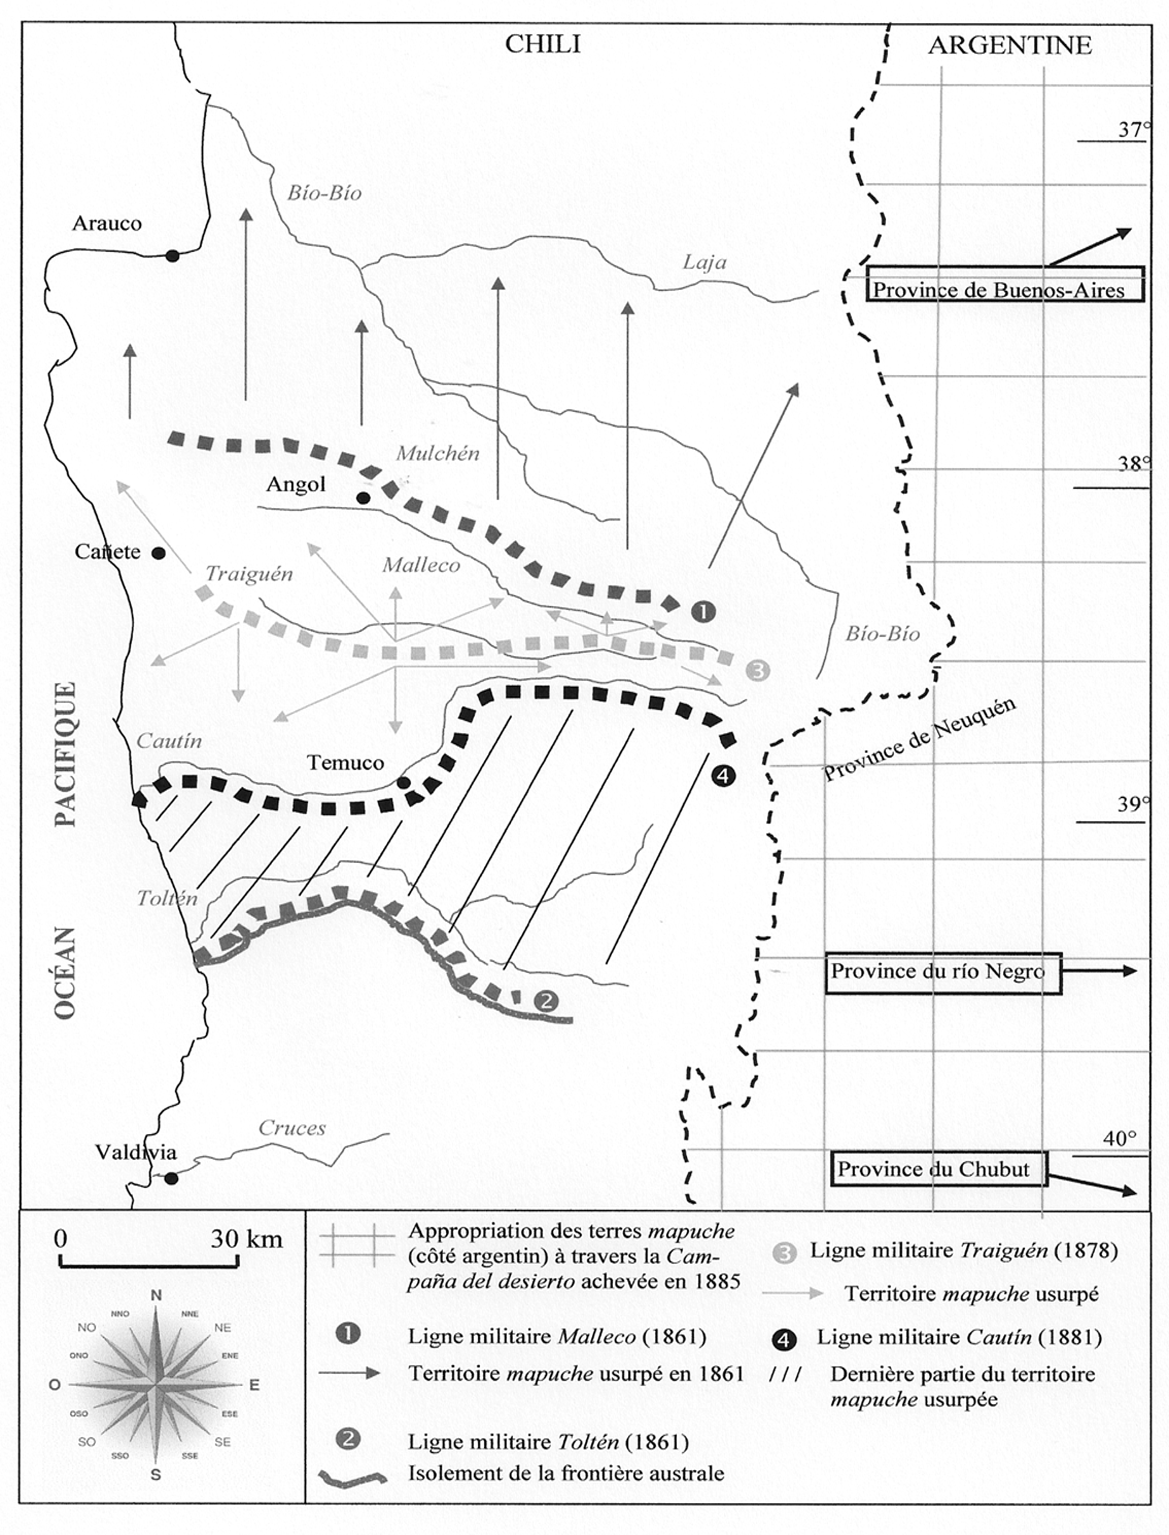
\includegraphics[width= 0.5\textwidth]{annexes/carte/carte_expansion.png}
	    \caption{Carte de l’usurpation progressive du territoire Mapuche (1810-1885)\protect\footnotemark}
	    \label{fig:my_label}
	\end{figure}
	\footnotetext{\cite{nouailleIndependanceChiliConsequences2012}}
	
	Cette répression s'intensifie à partir de 1859, après le soutien explicite de certains chefs mapuches auprès des révolutionnaires libéraux lors de l'insurrection de 1859 contre le gouvernement. En 1866, les premières lois d'occupation ont été adoptées en modifiant la nature du \enquote{territoire indigène} pour  \enquote{territoire de colonisation}. Elle entérine officiellement le processus colonial entrepris par l'État chilien avec la nomination de Cornelio Saavedra, initiateur de cette expansion, au poste d'intendant d'Arauco\footcite[p~.314]{bengoaMemoriaOlvidadaHistoria2004}. Celui-ci entama la fortification de la région tout en multipliant les lois facilitant l'appropriation des terres jusqu'au bord des rivières Malleco River et Toltén River. Durant ces 20 années, le conflit enferme progressivement le peuple Mapuche aux confins des terres araucaniennes et de la Cordillère des Andes, perdant ainsi 90,7\% de son territoire original\footcite[p~.350]{bengoaMemoriaOlvidadaHistoria2004}.
	
	Le conflit autour de l'Occupation de l'Araucanie qui dura jusqu'en 1881, n'est pas un épiphénomène au sein d'un processus d'extension territoriale et d'affirmation politique. Il est un tournant progressif majeur en enterrant définitivement une identité fondée sur un État-nation pluriel, comme nous l'évoque l'historien Pablo Mariman Quemenado: 
	
	\begin{quote}
	    \enquote{Il s'est terminé l'idée d'un État qui abhorre la diversité qui le constitue, fondant la relation et la situation coloniales avec des peuples désormais catégorisés comme "communautés indigènes"\footnote{\enquote{Concluida esta, se termina consumando la idea de un  Estado  que  abomina  de  la  diversidad  que  lo  constituye,  fundando  la  relación  y  situación  colonial  con  pueblos  que  fueron  categorizados  en  adelante  como  “comunidades indígenas”}\cite{quemenadoGeoestrategiaConflictoChileno2017a}}}
	\end{quote}
	
	\begin{figure}[p]
	    \centering
	    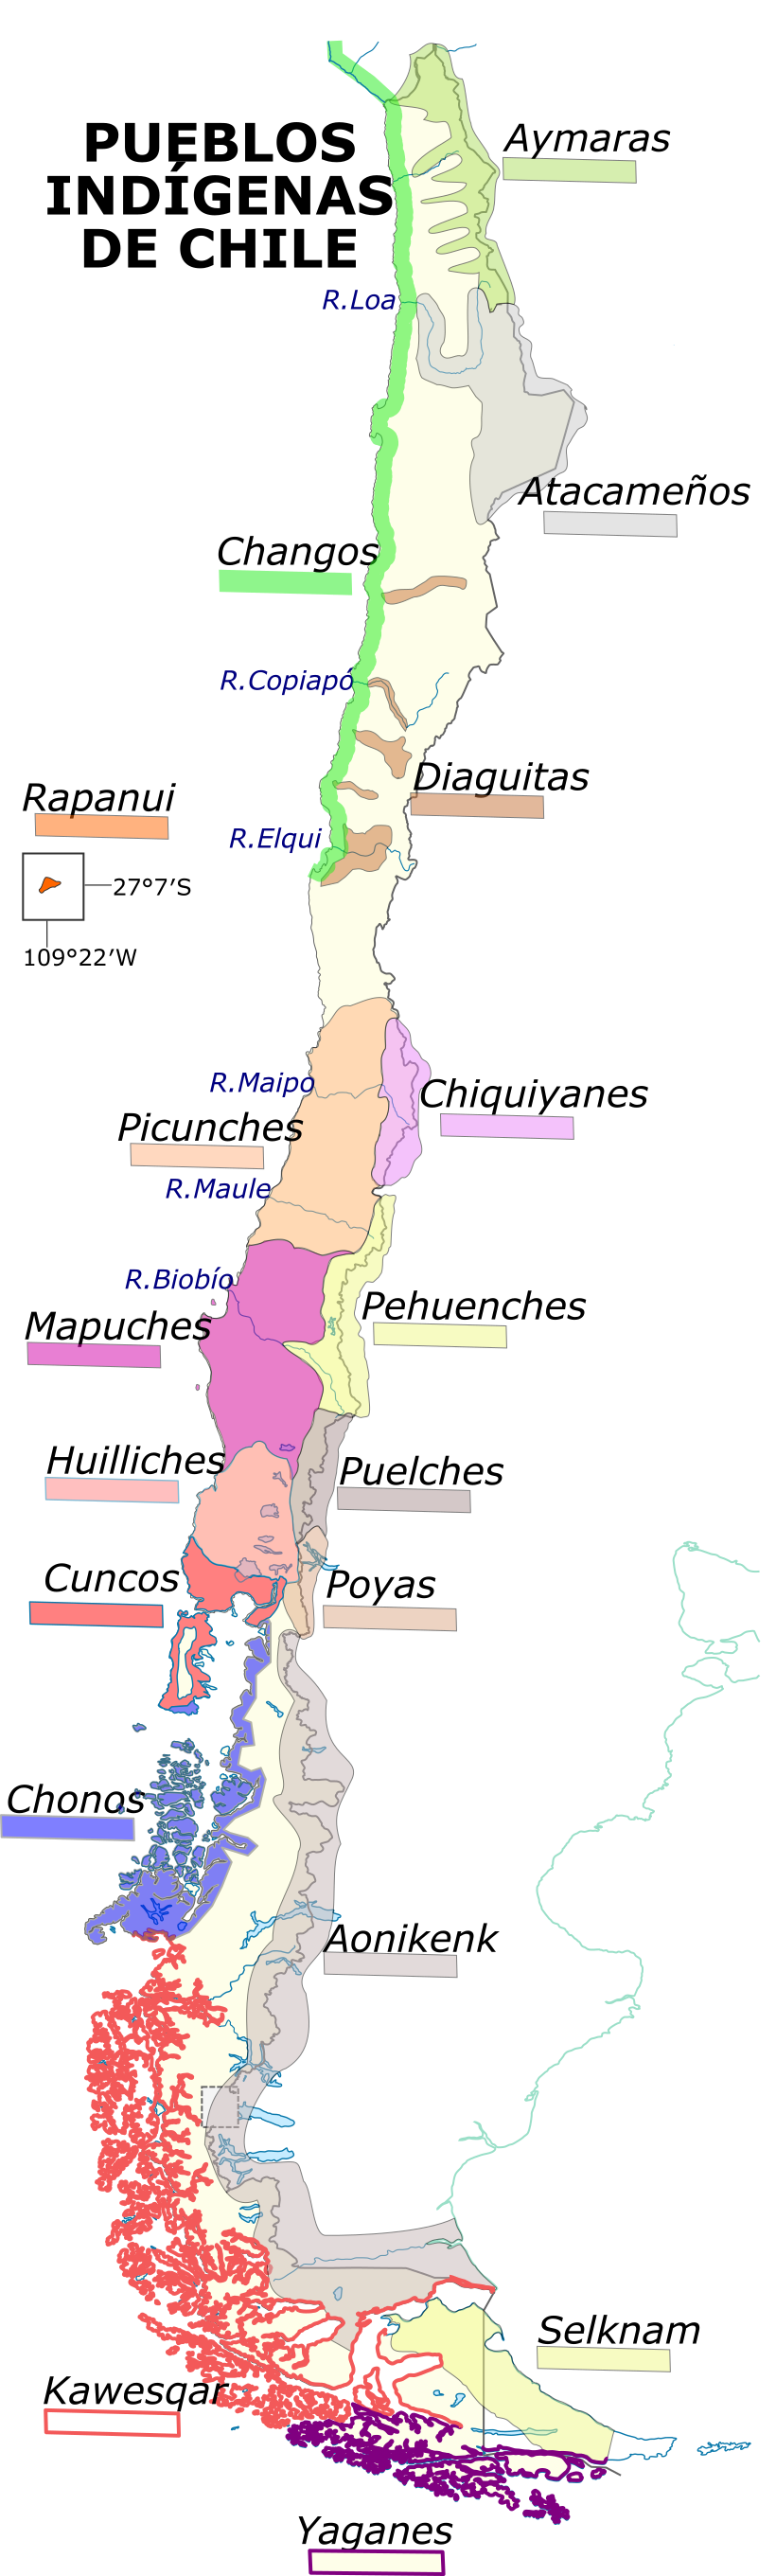
\includegraphics[width= 0.45\textwidth]{annexes/carte/carte_peuples.png}
	    \caption{Carte schématique des principaux peuples autochtones existants ou ayant existés au sein du territoire chilien actuel - \copyright Wikipedia}
	    \label{fig:carte_chili}
	\end{figure}
	
	\subsection{La question Mapuche : symbole des problèmes socio-politiques du Chili contemporain}
	
	À l'heure actuelle, la lutte pour la légitimité des droits territoriaux et politiques Mapuche est devenue un symbole de mobilisation ethno-sociale à la fois sur le plan national qu'international. Sa lutte singulière s’est progressivement transformée en une source d’inspiration culturelle inaltérable et presque romantique face à l'étatisme et la capitalisme néo-libéral\footcite{sepulvedaPaysMapucheTerritoire2012}.
	
	Dès 1910, un premier mouvement autochtone Mapuche se forme à travers le collectif \textit{Sociedad Caupolican de Defensa de la Araucanía}. Au cours du XX\textsuperscript{e} siècle, de nombreuses organisations politiques voient le jours avant de disparaître selon les tournants de l'histoire politique chilienne. Ce conflit latent accompagne au contraire le débat et les querelles sur fond d'inimitié ou au contraire de solidarité. Cette réclamation territoriale est devenue multiple et s'étend jusqu'aux territoires argentins, là où la culture et l'influence Mapuche demeure : \enquote{en renouant avec les connexions transandines de l’époque coloniale, le déploiement des systèmes circulatoires contemporains à l’échelle du cône sud-américain redonne une indéniable matérialité\footcite{sepulvedaPaysMapucheTerritoire2012}}.
	
	Si des territoires exclusifs et protégés ont été déterminés afin de reconnaître certains droits aux peuples indigènes présents sur le territoire chilien. Cette rédemption hésitante reste constamment sous le feu des critiques politiques et économiques. Aujourd'hui, si l'appartenance ethnique et les traditions culturelles se perpétuent, cette population est confrontée à de nombreux problèmes socio-économiques représentant environ un million de personnes\footcite{bengoaMapuchesHistoriaCultura2011}. En effet, la plupart des territoire hors réserves indigènes, restent soumis au monopole d'une grande industrie forestière, agricole et piscicole réfractaire face à la perte de leurs capitaux\footcite{andradeLuchaPorTerritorio2019}. Cette dépossession économique alimente les conflits locaux , mais aussi nationaux.
	
	Ces crispations sociales se sont exacerbées à partir des années 1990, où l'utilisation de la violence politique comme une pratique de contestation connaît un léger regain suite à la fébrilité de la loi Indigène de 1993. Au sein des sphères politiques et médiatiques se dresse progressivement une criminalisation de la lutte politique mapuche, dépeignant son intensification comme une menace contre l'État\footcite{carvajal-delmarCriminalisationConflitMapuche2014}. Sous fond d'une politique de discrimination raciale, la politique répressive de la contestation va être étendue par l'emploi de la loi antiterroriste promulguée en 1984 sous de la dictature de Pinochet\footcite{carvajal-delmarCriminalisationConflitMapuche2014}. 
	
	Depuis le début des années 2000, l'État chilien prétend mettre fin avec cette politique répressive des contestations avec un peuple chilien qui souhaite démontrer une plus large volonté de conciliation\footcite{nouailleIndependanceChiliConsequences2012}. Néanmoins, les tensions localisées persistent dans la région de Biobío et de l'Araucanie. Certains territoires de la région de Wallmapu sont encore récemment soumis à un état d'exception juridique et une militarisation de la région. Ces tensions encore très vives démontrent la continuité d'un conflit historique dont les enjeux sociaux et politiques persistent.
	    
    \subsection{La sous-collection de l'\textit{Araucania}}
    
    La "Colección Manuscritos" est l'un des fonds les plus importants détenus par le centre \gls{acab}, avec plus de 2200 documents manuscrits datant de 1642 à 1952. Cette collection s'est progressivement constituée grâce à des dons d'universitaires et de politiciens liés à l'Universidad de Chile, mais aussi grâce à diverses acquisitions au cours du XX\textsuperscript{e} siècle\footnote{Voir le registre de l'inventaire de "Colección Manuscritos", \textit{Archivo Central Andrés Bello}, url: \url{http://archivobello.uchile.cl/content/Registro\%20Guia/2016/enero/registro_guia_coleccion_manuscritos.pdf}, consulté le 02/08/2022.}. Ces documents se regroupent autour de différentes grandes thématiques de l'histoire du Chili et dont une grande partie a été produite par des figures éminentes de la vie politique, militaire et intellectuelle (Andres Bello, Manuel Montt, etc.). De par le prestige de ses producteurs et de l'importance historique de ces documents, ce fonds a été classé comme \enquote{Monument historique} par le décret n°295-2009 du ministère de l'Éducation du Chili durant l'année 2009\footnote{Décret n°295-2009 du ministère de l'Éducation du Chili, \textit{Declara Monumento Nacional en la categoría de Monumento Histórico las colecciones Neruda, Americana y Manuscritos, pertenecientes al Archivo Central Andrés Bello, de la Universidad de Chile}, promulgé le 5 août 2009 et publié le 5 septembre 2009}.\newpar
    
    Les archives concernant l'Occupation de l'Araucanie en constituent une part essentielle. Ce sous-fonds spécifique autour des archives de l'Occupation de l'Araucanie a été inventorié partiellement à partir de la fin des années 2000, dans le prolongement de la création de la collection "Colección Manuscritos". Cette première classification et la restauration parcellaire et progressive à permis de mettre à jours des centaines d'archives, suscitant l'intérêt des milieux scientifiques et patrimoniaux. 
    
    En 2013, un important  travail de numérisation a été mis en place, axée sur la pacification de l'Araucanie, grâce à l'octroi d'un fonds du programme ADAI (Apoyo al Desarrollo de los Archivos Iberoamericanos) qui permettra la numérisation de 249 documents, pour un total de 530 pages. Ce programme a permis de donner suite à une première transcription manuelle les années suivantes. Ce projet d'édition numérique s'inscrit donc dans cette continuité en s'appuyant sur les différents travaux précédents.\newpar
    
    En observant plus en détail, les archives numérisées du sous-fonds de la "Colección Manuscritos", nous pouvons remarquer que l'essentiel de l'activité de la production documentaire se concentre sur la période 1859-1860. Cette période de transition se situe plus exactement entre la fin des \enquote{guerras civiles "montistas"} (1850-1859) dont l'année 1859 est marquée par le soulèvement général de nombreuse tribut mapuche. Cette répression fut suivi d'une campagne de militarisation et pacification de la région dirigée par Nicolas Saavedra. Il mit ensuite en œuvre du plan d'occupation de la région Biobío à partir de 1861\footcite[p.~165-171]{bengoaHistoriaPuebloMapuche1987}. Le recensement de l'activité se concentre surtout la fin de l'année 1859 à février 1860, avec un certain regain pour le mois de juin et octobre 1860 (voir annexe A, figure \ref{fig:day_activities}). Toutefois, on retrouve de nombreux documents s'éparpillant sur l'ensemble de la seconde moitié du XIX\textsuperscript{e} siècle, bien qu'une part essentielle n'est pas encore pu être numérisé.


	\section{La construction d'un jeu de donnée : vers une utilisation tout terrain}
	\sectionmark{La construction d'un jeu de donnée}
	
	\subsection{Préparation des données numérisées et leur inventorisation}
	
	La constitution d'un jeu de données homogène et structuré a été une étape importante dans la préparation, à la fois pour s'immerger et comprendre les informations et les subtilités qui en résident. Comme nous l'avons vu précédemment, ce corpus documentaire autour des archives de l' \enquote{Occupation de l'Araucanie} a déjà été le fruit d'un long travail de révision et d'inventorisation minutieux de la part de l'équipe en charge du processus d'archivage. L'ensemble des informations ont été recueilli sous la forme d'un tableur Excel (Word office) en rassemblant des données sur chaque pièce de ce fonds partiel : date, côtes et identifiant des numérisations, indications géographiques et humaines, type, nombre.
	
	Toutefois, un certain nombre d'éléments ne furent pas adaptés à une exploitation machine, mais davantage à une interprétation humaine. Un travail de réconciliation, d'uniformisation et d'épuration des données a été mis en place en extrayant les données sous le format \gls{csv}. Ce format fut ainsi interprétable par le logiciel \texttt{Dataiku DSS}. Cette plateforme de développement intégré est destinée à l'ensemble des besoins dans le cadre traitement et analyse de la donnée. \texttt{Dataiku} a ainsi permis le retypages des données initiales, mais aussi de quantifier les archives numérisées\footnote{L'ensemble du flux de travail est disponible à l'adresse suivante : \url{https://github.com/Proyecto-Ocupacion-Araucania-UChile/Data_preparation}.}. Les enjeux de ce traitement se déclinent en trois objectifs: \\
	\begin{itemize}
	    \item Inventaire des fichiers permettant de vérifier si certains fichiers ne sont pas manquants. Il fut ensuite possible de les classer en fonction de la nature et la typologie des documents.
	    \item La conversion des images. À l'origine, le service de numérisation de \gls{acab} a produit les images sous le format \gls{tiff} (à 1200 dpi) permettant une qualité maximale. C'est un format d'image matricielle permettant de ne pas compresser l'image et ainsi de garder celle-ci la plus authentique possible en limitant la perte des données. Ce standard au sein des institutions patrimoniales reste en revanche un objet extrêmement lourd avec une moyenne autour de 60 mo (mégaoctets). Des projets similaires ont démontré qu'une telle qualité n'était pas nécessaire et qu'une image compressée est amplement suffisant\footcite{n.c.ExperimentationsLECTAUREP, chiffoleauDAHNProjectDigital2022}. Ce script shell a permis d'automatiser la conversion de l'ensemble des images vers le format \gls{jpg} \footnote{voir annexe \ref{code:shell_img}.}.
        \item Faciliter l'interprétation des données dans un travail d'analyse ou comme support à la production de métadonnées lors de son édition. \\
	\end{itemize}
	
	Cette première étape permet de mettre en place une stratégie, évolutive néanmoins quant à la constitution du set de données mais aussi sur la mise en place de certains stratagèmes afin de récupérer la donnée le plus efficacement possible avec une perte marginale. Notre jeu de données disponibles est en effet assez restreint au vue de certains autres projets de reconnaissance d'écritures manuscrites; il est donc impératif de maximiser celle-ci. Il faut pour cela essayer de sélectionner les plus qualitatives, représentatives et homogènes possibles. En observant les différents graphiques, on peut apercevoir la sur-représentation des lettres, et secondairement les notes manuscrites au sein du corpus documentaire (graphique \ref{fig:percent_type}). Nous avons donc pris la décision de centraliser les efforts sur ces deux typologies, avant d'étendre le processus en fonction du résultat. Dans un deuxième temps, la distribution des archives montrent une grande pluralité d'auteurs au sein de ce fonds. En revanche, six personnes se manifestent comme amplement plus prolifiques que la moyenne (graphique \ref{fig:author_distribution}).
	
	\subsection{Constitution d'un corpus interopérable}
	
	À la suite de différentes recherches sur l'existence de \textit{dataset}, il est rapidement apparu que la langue espagnole occupait une position plus marginale dans les domaines de la recherche et de l'ingénierie autour de l'\gls{htr}. Si quelques projets ont été mis en place, l'essentiel se tourne vers la recherche fondamentale sur les réseaux neuronaux ou ne sont pas librement accessibles\footnote{À cet égard, on peut remarquer que l'\textit{Universitat Politècnica de València} est particulièrement actif à ce sujet comme le démontre les récentes publications : \cite{granellTranscriptionSpanishHistorical2018, espana-boqueraSpanishDatasetReproducible2022}}. De la même manière, des plateformes telles que \texttt{HTR-United} ne recensent que très peu de données disponibles sur cette langue, ou alors inadaptées à la construction d'un modèle adapté \gls{acab}.
	
	Face à ces premiers constats, l'édification d'un modèle dédié paraît donc indispensable, ce qui nécessite de construire au préalable un lot de données d'entraînement. Le premier enjeu de cette automatisation est en réalité triple puisqu'il s'agît d'établir les règles structurelles, épistémologiques et analytiques des transcriptions et de l'interprétation machine. La qualité des données utilisées et leur cohérence sont à la source du succès des prédictions, dans le cadre d'un apprentissage machine supervisée\footnote{Cf. chapitre 4}.
	
	En effet, des erreurs d’acquisition ou de transformation liées à des fautes humaines ou techniques peuvent considérablement ralentir, voire mettre à mal la poursuite du projet. La performance de cette chaîne de traitement, mais aussi la réutilisation à moindre coût énergétique et de temps va dépendre d'une analyse préalable des sources. La dimension d'interopérabilité doit permettre l'utilisation multiple de ce jeu de donnée sur l'ensemble du processus de traitement : segmentation, reconnaissance d'écriture manuscrite et reconnaissance d'entités nommées. \newpar
	
	La constitution d'un corpus documentaire dans le but de l'exploiter dans un projet d'édition numérique, nécessite donc un set quantitatif, mais surtout qualitatif afin de procéder à une restitution de l'information la plus complète possible. Si l'aspect quantitatif semble de prime abord plus que négligeable en comparaison d'autres projets, plusieurs études ont démontré l'efficacité de jeu de données à la taille plus modeste tout en permettant un coût marginal\footcite{sanchezSetBenchmarksHandwritten2019}. La principale difficulté réside dans la segmentation et non la reconnaissance de caractères. Par la suite, les chercheurs Phillip Benjamin Strobel, Simon Clematide et Martin Volk ont démontré qu'un jeu de données de plus de 50 pages était suffisant pour avoir des prédictions pouvant être qualifiées de bonnes sur le moteur \gls{kraken} \footcite{strobelHowMuchData2020}.
	
	Au vu de nos précédentes analyses, il est frappant de voir la forte hétérogénéité de notre corpus ce qui induit la nécessité d'un modèle polyvalent en conséquence d'un fonds extrêmement composite. 
	Ces données préliminaires vont ainsi révéler un ensemble de facteurs et problématiques à prendre en compte afin de tendre vers une automatisation la plus efficiente possible\footcite{chagueDeuxSieclesSources2019a}.
	

    \begin{table}[h!]
    \centering
    \begin{adjustbox}{max width=1\textwidth}
    \begin{tabular}{|c|c|ccc}
    \hline
    \multicolumn{1}{|l|}{\textbf{Nom}} & \multicolumn{1}{l|}{\textbf{Pages}} & \multicolumn{1}{l|}{\textbf{Dates extrêmes}}       & \multicolumn{1}{l|}{\textbf{Particularités}}                                                         & \multicolumn{1}{l|}{\textbf{Données test}} \\ \hline
    Cornelio, Saavedra                 & 43                                              & \multicolumn{1}{c|}{nov. 1859 - août 1877}     & \multicolumn{1}{c|}{style propre, bon état, présence de notes post-scriptum}                         & \multicolumn{1}{c|}{Non}                   \\ \hline
    Avello, Juan                       & 12                                              & \multicolumn{1}{c|}{nov. 1859 - nov. 1860} & \multicolumn{1}{c|}{style propre, quelques feuilles abimées, présence de notes post-scriptum}        & \multicolumn{1}{c|}{Non}                   \\ \hline
    Díaz, José Del Carmen              & 21                                              & \multicolumn{1}{c|}{déc. 1859 - mars 1860}     & \multicolumn{1}{c|}{style propre parfois condensé, bon état}                                         & \multicolumn{1}{c|}{Non}                   \\ \hline
    Escala, Manuel Segundo             & 13                                              & \multicolumn{1}{c|}{nov. 1859 - nov. 1860} & \multicolumn{1}{c|}{style très propre, bon état}                                                     & \multicolumn{1}{c|}{Non}                   \\ \hline
    García Videla, Daniel              & 8                                               & \multicolumn{1}{c|}{mai 1860 - juin 1860}          & \multicolumn{1}{c|}{style très propre, bon état}                                                     & \multicolumn{1}{c|}{Non}                   \\ \hline
    Pérez Rosales, Vicente             & 12                                              & \multicolumn{1}{c|}{fév. 1860 - nov. 1860}  & \multicolumn{1}{c|}{style parfois hésitant et condensé, bon état}                                    & \multicolumn{1}{c|}{Non}                   \\ \hline
    Sepúlveda, José                    & 8                                               & \multicolumn{1}{c|}{déc. 1859 -nov. 1860}  & \multicolumn{1}{c|}{style intermédiaire, quelques feuilles abimées, présence de notes post-scriptum} & \multicolumn{1}{c|}{Oui}                   \\ \hline
    Villalón, Vicente                  & 22                                              & \multicolumn{1}{c|}{nov. 1859 - nov. 1859} & \multicolumn{1}{c|}{style propre, parfois effacé, présence de notes post-scriptum}                   & \multicolumn{1}{c|}{Non}                   \\ \hline
    Contreras, Juan                    & 16                                              & \multicolumn{1}{c|}{mars 1860 - juin 1860}         & \multicolumn{1}{c|}{style convenable, quelques feuilles légèrement abimées}                          & \multicolumn{1}{c|}{Non}                   \\ \hline
    Echantillon composite              & 25                                              & \multicolumn{1}{c|}{nov. 1859 - nov. 1859} & \multicolumn{1}{c|}{16 mains, bon état}                                                              & \multicolumn{1}{c|}{Non}                  \\ \hline
    \multicolumn{1}{|l|}{TOTAL}        & \multicolumn{1}{l|}{180}                        & \multicolumn{3}{l}{\cellcolor[HTML]{C0C0C0}{\color[HTML]{9B9B9B} }}                                                                                                                                    \\ \cline{1-2}
    \end{tabular}
    \end{adjustbox}
    \caption{Détails du jeu de données sélectionné}
    \label{tab:dataset}
    \end{table}

	
	Cet échantillonnage a été réalisé, de manière progressive et empirique, à partir de multiples mains en en s'appuyant sur le schéma du projet \enquote{LECTAUREP\footnote{\textit{LECTure Automatique de REPertoire}; pour plus d'informations, voir \url{https://lectaurep.hypotheses.org/}.}} mis en place par l'équipe ALMAnaCH de l'\gls{inria}. En premier lieu, le corpus s'est construit autour de plusieurs lots alternant entre 10 et 15 numérisations par auteur au nombre 6. Petit à petit, d'autres transcriptions ont été agrégées au lot déjà existant. À partir de là, la stratégie d'apprentissage s'est appuyée sur un lot conséquent d'une main unique (plus de 40 documents), un nombre de mains variables avec une production documentaire modérée voire élevée et un lot s'appuyant sur de très courtes transcriptions venant de nombreuses mains différentes. Ce choix vise à permettre un apprentissage stylistique et graphologique extrêmement varié et ainsi permettre la production d'un modèle le plus polyvalent possible en s'appuyant sur une méthodologie dite générique \footcite{pincheCREMMALabProjectHandwritten2022}.
	
	\section{Disséquer l'image et reconstruire l'information : une étape préliminaire à la transformation éditoriale}
	\sectionmark{Disséquer l'image et reconstruire l'information}
	
	La segmentation est un principe général du traitement et de l'analyse optique d’une image afin d’obtenir la reconnaissance des régions et des lignes d’écriture. De nombreux projets d'éditions numériques s'appuient justement sur cette reconnaissance pour transformer une image brute en édition numérique native.
	La mise en place de ce procédé nécessite au préalable une clarification des enjeux sémantiques et  en définissant au préalable un protocole d'annotation et de transcription. L'emploi d'une telle méthode doit ainsi permettre une automatisation de l'extraction de l'information dans son contexte, s'apparentant à une analyse diplomatique, et vérifier la solidité du processus de transformation.
	
	\subsection{Ontologie d'une procédure de segmentation d'un document}
	
	Comme nous pourrons l'observer plus en détail au sein du chapitre 4, l'un des principes novateurs de l'\gls{htr} est l'analyse de la mise en page (\textit{layout analysis}) dans le processus de reconnaissance des écritures. Cette étape consiste à détecter les zones d’intérêts dans une image, les différencier et spécifier leur intérêt : ligne de texte, régions, réclames, marges. On déconcentre le processus d'apprentissage\footcite[p.~25]{noemieOCRHTRGraphie2022}. C'est-à-dire que l'écriture n'est plus l'unique point de fixation, c'est désormais l'ensemble de la page qui est prise en compte pour en attraper l'information substantielle.
	
	Cette technologie dans le domaine de la reconnaissance d'écriture offre ainsi un double avantage : la reconnaissance d'écriture manuscrite complexe et une reconnaissance morphologique de l'image au travers de son processus de segmentation. Ces régions et ses bases de lignes vont permettre de recontextualiser le texte au moyen d'une structuration sémantique de la donnée. L'intérêt est de conserver la structure diplomatique initiale en vue de l'encodage éditorial du texte. 
	
	\begin{figure}[h!]
	    \centering
	    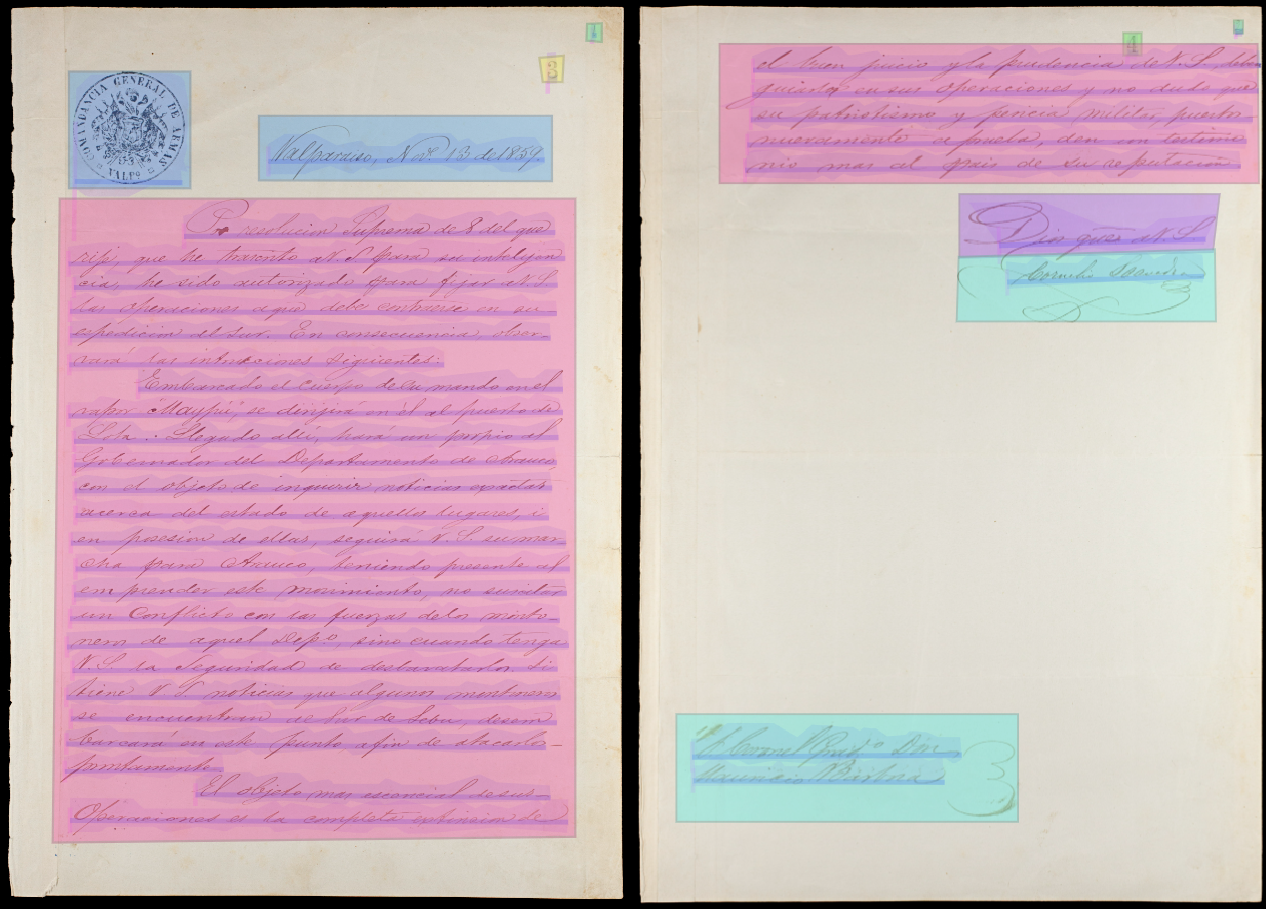
\includegraphics[width = 0.90\textwidth]{annexes/img/segmentation_img.png}
	    \caption{Démonstration d'une segmentation d'image sur l'application \gls{eScriptorium}}
	    \label{fig:segmentation}
	\end{figure}
	
	Comme nous pouvons le constater à travers de cette image reprenant la codification des régions, la stratégie adoptée s'est appuyée sur une délimitation sémantique, au détriment de la segmentation centrée sur une perception visuelle (voir figure \ref{fig:segmentation}). Si cette méthode permet de conserver au maximum le sens de la donnée initiale, elle se fait au détriment d'une cohérence visuelle. On peut observer que de nombreuses lignes sont régulièrement rapprochées entre elles, voir superposées. Cette structuration graphique peut donner lieu à un certain nombre de confusions lors du processus de segmentation machine.
	
	D'autres projets d'édition numérique ont eu pour enjeux la structuration de données autour de nature similaire à celui du projet du centre \gls{acab}. Les travaux de Floriane Chiffoleau et Anne Baillot sur le projet de \gls{dahn} ont ainsi pu expérimenter l'élaboration d'une ontologie des corpus littéraires et mettre à disposition des \textit{guidelines} décrivant les principes généraux\footcite{chiffoleauDAHNProjectDigital2022}. Sur ce constat et en s'appuyant sur une première appréciation du corpus documentaire, une ontologie a pu être dessinée dans le but d'annoter les différentes régions et les différentes lignes détectées . Celle-ci se décline sur 14 types de régions et 3 types de lignes présentées ci-dessous: \\
	
	\begin{itemize}
	    \item \textbf{Régions} :
	    \begin{enumerate}
	        \item \textit{CustomZone:Address} -- Zone indiquant le destinataire
	        \item \textit{CustomZone:Dateline} -- Zone indiquant le contexte d'écriture (date et lieu)
	        \item \textit{CustomZone:Object} -- Zone indiquant l'objet du document
	        \item \textit{MainZone:SaluteConclude} -- Zone indiquant la salutation conclusive
	        \item \textit{MainZone:SaluteIntro} -- Zone indiquant la salutation introductive
	        \item \textit{MainZone:Text} -- Zone indiquant le corps du texte
	        \item \textit{MarginTextZone:commentary} -- Zone indiquant les commentaires en marge du texte
	        \item \textit{MarginTextZone:note} -- Zone indiquant les notes additionnelles
	        \item \textit{NumberingZone:id} -- Zone indiquant le numéro d'identification (\textit{a posteriori})
	        \item \textit{NumberingZone:other} -- Zone indiquant un numéro additionnel (\textit{a posteriori})
	        \item \textit{NumberingZone:page} -- Zone indiquant le numéro de page (\textit{a posteriori})
            \item \textit{QuireMarksZone:signature} -- Zone indiquant la signature de l'auteur
            \item \textit{StampZone:graphic} -- Zone indiquant une estampille graphique
            \item \textit{StampZone:manuscript} -- Zone indiquant une estampille manuscrite
	    \end{enumerate}
	    \item \textbf{Lignes} :
	    \begin{enumerate}
	        \item \textit{DefaultLine} -- Ligne par défaut
	        \item \textit{InterlinearLine:commentary} -- Ligne indiquant un commentaire entre deux lignes
	        \item \textit{InterlinearLine:correction} -- Ligne indiquant une correction entre deux lignes\newpar
	    \end{enumerate}
	\end{itemize}
	
	Cette composition doit permettre la description de trois natures de documents : les lettres, les notes et les circulaires. Si ces trois objets ont une portée sémantique différente, il en reste que cette sélection possède des caractéristiques structurelles très similaires pouvant rapidement être associées et ainsi alléger l'ontologie. Comme nous pouvons le constater, l'ontologie a été amplement enrichie au modèle initial du projet \gls{dahn}. Les particularités de notre corpus hétérogène et l'alignement sur la méthodologie de l'initiative \gls{segmonto} ont amené à reconsidérer et remodeler cette base ontologique.
	
	Avant tout créé pour parachever l'étude des manuscrits médiévaux et des imprimés anciens, le projet \gls{segmonto}, né en 2021, est une réponse de différents chercheurs aux besoins d'un modèle efficace et de faire coexister la taxonomie des numérisations et l'approche éditoriale du texte\footcite{gabaySegmOntoCommonVocabulary2021a}. Cette initiative universitaire offre un vocabulaire contrôlé permettant une description graphique d'un texte sous sa forme la plus essentielle. L'ontologie est construite autour de 15 zones principales et 6 types de lignes; auxquelles peut être additionné un complément d'information par l'utilisation des signes \enquote{:} ou \enquote{\#} en suffixe\footcite{gabaySegmOntoControlledVocabulary2021a}. En outre, l'utilisation de ce lexique renforce l'interopérabilité des données entre les projets et ainsi permettre non seulement de créer des outils numériques pérennes, mais aussi de donner la possibilité de leur réutilisation.
	
	\subsection{\texttt{XML-ALTO}: un encodage structuré adapté à l'océrisation}
	
	Afin de comprendre la portée et l'utilisation possible des données possibles, il est nécessaire de comprendre le format d'expression de celle-ci. Au sein de l'univers de la reconnaissance d'écriture, il y a deux grands standards \gls{xml} qui accompagnent principalement et structurent les résultats \gls{ocr} : le format \gls{xml} \gls{alto} et le format \gls{page}. Dans notre cas, nous avons choisi de nous appuyer sur le premier standard qui est le plus couramment utilisé, en particulier au sein des institutions patrimoniales\footcite[p.~74]{caronFormatsDonneesPour2021}. Il offre deux avantages : la conservation des données coordonnées géométriques et la superposition de l'image.
	
	Pour revenir à la base, \gls{xml} est un métalangage de structuration de données à balise publié en 1999 par le consortium \gls{w3c}. L'atout principal de ce langage est sa grande permissivité et sa grande extensibilité avec son système à chevron. \gls{alto} est un standard dérivé de \gls{xml} défini par un schéma aujourd'hui maintenu par la \textit{Library of Congress}\footcite[p.~74]{caronFormatsDonneesPour2021}. Il a été développé à partir de 2004 afin de répondre au besoin naissant de l'\gls{ocr} afin de pouvoir décrire la mise en page des documents et assurer la conservation à long terme des données. \newpar
	
	\begin{listing}
	        \begin{minted}{xml}
	        <TextBlock HPOS="842"
                   VPOS="3078"
                   WIDTH="1161"
                   HEIGHT="271"
                   ID="eSc_textblock_493a77e7"
                   TAGREFS="BT3114">
          <Shape><Polygon POINTS="883 3128 842 3342 2003 3349 1999 3078"/></Shape>
          
          
          <TextLine ID="eSc_line_1f8ebff3"
                    TAGREFS="LT1061"
                    BASELINE="1264 3203 1951 3209" 
                    HPOS="1261"
                    VPOS="3079"
                    WIDTH="690"
                    HEIGHT="156">
            <Shape><Polygon POINTS="1264 3203 1264 3140 1315 3140 1318 3140 1388 3079 1388 3079 1391 3079 1391 3079 1391 3079 1395 3079 1395 3079 1395 3079 1398 3079 1398 3079 1401 3079 1468 3095 1573 3079 1573 3079 1576 3079 1576 3079 1576 3079 1579 3079 1579 3079 1579 3079 1703 3140 1789 3111 1792 3111 1792 3111 1792 3111 1795 3111 1795 3111 1798 3111 1798 3111 1798 3111 1801 3111 1801 3111 1801 3114 1833 3143 1833 3146 1951 3146 1951 3209 1948 3235 1261 3235"/></Shape>
	    <String CONTENT="⁋J del C. Díaz"
                    HPOS="1261"
                    VPOS="3079"
                    WIDTH="690"
                    HEIGHT="156"></String>
          </TextLine>

          
        </TextBlock>
            \end{minted}
        	\caption{Structuration d'un fichier ALTO}
        	\label{code:alto_struct}
    \end{listing}
    
    Un fichier XML ALTO est composé de trois sections principales : \balise{Description} permettant de décrire les métadonnées, \balise{Styles} renseigne les données de styles (police, etc.) et \balise{Layout} est la section décrivant les différents éléments de mise en page. Dans notre cas, les deux éléments les plus intéressants sont les éléments \balise{TextBlock} et \balise{TextLine} comme nous pouvons constater à travers cet extrait du code sources d'un résultat \gls{htr} (voir le code \ref{code:alto_struct}). L'élément \balise{TextBlock} indique les différentes données liées à la région dont l'attribut \attribut{TAGREFS} affiche la référence de la région, les autres attributs sont dédiés aux informations géométriques condensées. Le sous-élément \balise{Polygon} permet de décrire le dessein du masque de la zone sur l'axe X/Y. De la même manière, \balise{TextLine} est réservé aux données autour de la ligne. Au sein du sous-élément \balise{String}, l'attribut \attribut{CONTENT} rend compte de la transcription effectuée. \newpar
    
    Récemment un certains nombres d'outils ont été mis en place afin d'appuyer la solidité des données. Dans notre cas, la jeune application HTRVX développée et promue par HTR-United a permis de vérifier le schéma des données produites, la bonne concordance entre les zones et les lignes et de valider l'utilisation du vocabulaire SegmOnto\footcite{clericeHTRUnitedHTRVXHTRVX2022}. De ce fait, il fut très facilement possible de l'intégrer au sein du \textit{workflow} \gls{github} afin de vérifier l'apport de nouvelles de données et la bonne synchronisation entre elles.
	
	\subsection{Définir un protocole de transcription et d'annotation}
	
	Au cours de la préparation de données, l'ensemble des différentes transcriptions ont été effectuées sur l'application \gls{eScriptorium} afin d'en extraire des fichiers \gls{alto} exploitables lors de nos futurs entraînements. Cette phase s'est appuyée sur la première approche de Cecilia del Carmen Ramallo Díaz et son analyse des sources autour de l'Araucanie\footcite{carmenramallodiazdelTranscripcionDocumentosSerie2014}. Néanmoins, les transcriptions des documents ont été faites à travers une modernisation de la langue. Cela reste un frein majeur qui a nécessité de s'employer à de nouvelles transcriptions littérales.
	
	Au cours de la première phase, un ensemble de stratagèmes a été mis en place afin de récupérer un maximum de particularités depuis le texte original. Il s'agit des mots soulignés, barrés ou directement corrigés, des caractères illisibles ou partiellement lisibles et enfin des lettres suscrites. L'idée initiale était de pouvoir récupérer les différentes données et leurs évolutions grâce à l'aide d'un ensemble d'\gls{regex}. Une \gls{regex}, comme son nom l'indique, est un motif de caractères permettant de capturer ou échapper un à plusieurs éléments souhaités. Elle s'appuie sur une syntaxe particulière permettant de décrire la fonctionnalité souhaitée. Par exemple, pour récupérer le contenu d'un mot barré tel que \sout{Saavedra} signalé sous la forme \verb/*Saavedra*/, cela se traduitpar le motif suivant : \verb/\*([A-Za-zÀ-ÖØ-öø-ÿ -]+)\*/.
	
	Toutefois au vu des difficultés apparentes de l'interprétation machine lors des premiers essais effectués, il a été choisi de considérablement restreindre la codification des transcriptions. Une simplification qui s'est appuyée sur la méthodologie employée par le projet \gls{lectaurep}\footcite{durandNotairesParisRepertoires2021}. Si la première des raisons s'explique par l'intention d'optimiser les résultats, l'autre facteur était de pouvoir s'aligner sur les données du projet afin de les agréger à notre corpus et donc multiplier les données utilisables. Ainsi, seulement trois règles ont été appliquées:
	
	\begin{itemize}
	    \item lettre suscrite : \^e
	    \item mot illisible : xxx
	    \item nouveau paragraphe : \P.
	\end{itemize}
	
	 Cette dernière règle a été ajoutée afin de pouvoir délimiter plus facilement les différents paragraphes lors du processus d'édition. Les différentes expériences \gls{htr} ont démontré le besoin de simplifier les différentes règles de transcriptions afin d'être le plus optimal possible. Toutefois, l'utilisation du pied-de-mouche renversé n'a pas été conservée lors de la récupération des données sous un format texte (txt)\footcite{humeauPreprocessingHTR2022}.
	 
	 \begin{figure}[h!]
	     \centering
	     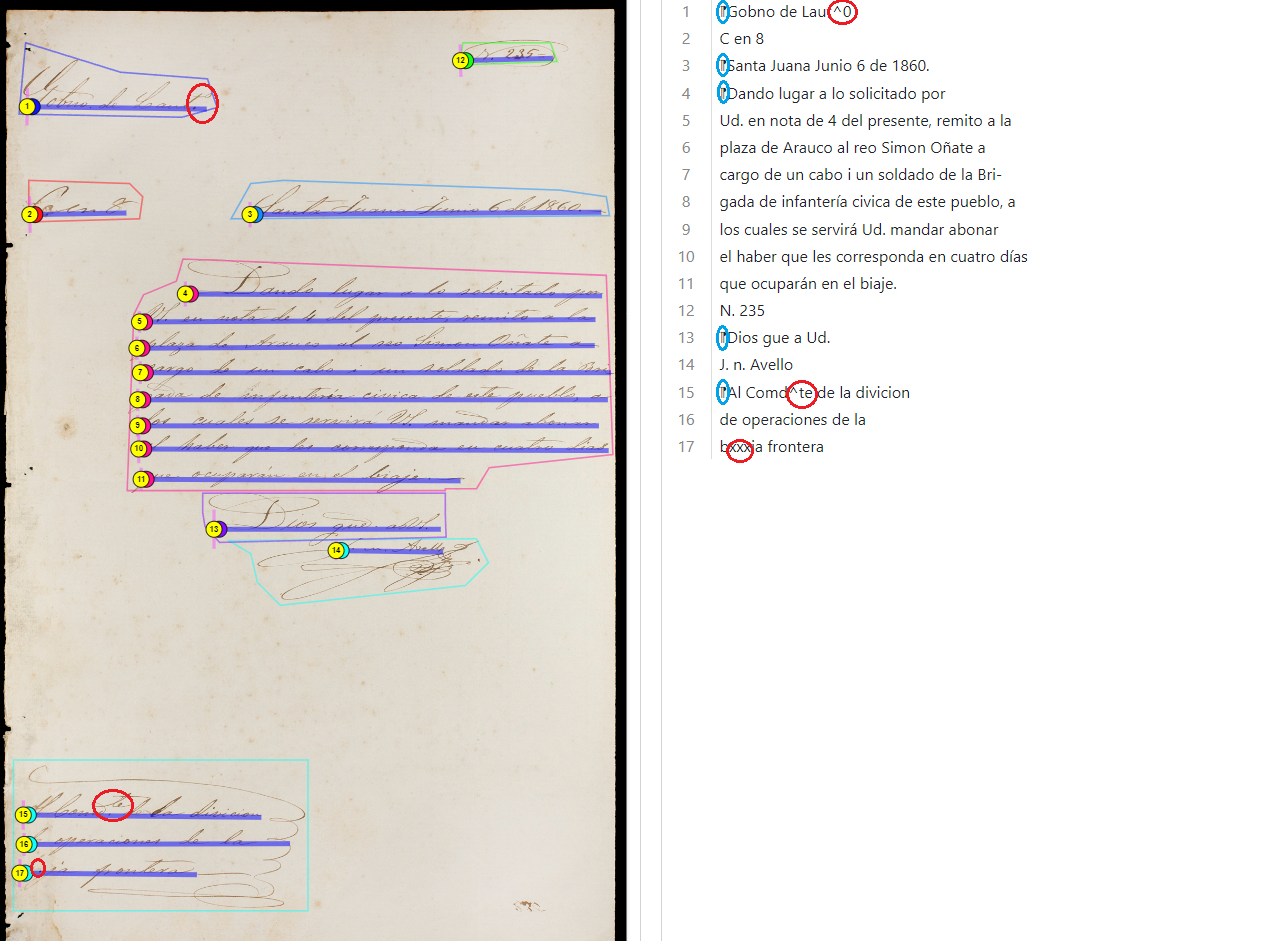
\includegraphics[width = 1.1\textwidth]{annexes/img/trans_rules.png}
	     \caption{Visualisation des règles de transcription}
	     \label{fig:transcription}
	 \end{figure}
	
	\section{Les enjeux du droit du patrimoine et de l'\textit{open data} au Chili}
	
	De nos jours, l'\textit{Open data} est devenu un enjeu majeur des institutions patrimoniales en permettant de faciliter l'accessibilité, le partage et la valorisation des données produites. Un mouvement scientifique est né autour de la volonté d'ouvrir la donnée afin de : \enquote{rendre la science plus accessible, démocratique, transparente et bénéfique pour tous\footcite{OpenScienceLatin2020}}. Une note de l'UNESCO (Organisation des Nations unies pour l'éducation, la science et la culture) révèle cet engouement général en Amérique latine afin de faire face aux problèmes d'accès aux ressources scientifiques, mais aussi à la valorisation de leur propres travaux\footcite{OpenScienceLatin2020}. 
	Toutefois, l'\textit{Open data} reste confronté à de nombreux besoins scientifiques, économiques et techniques et juridiques\footcite{jacqueminLibreAccesDonnees2019}. À travers ces observations, il s'agît de revenir sur les défis que traverse le développement d'un projet numérique autour des archives chiliennes.
	
	\subsection{Retour sur la législation des archives au Chili}
	
	En 2019, Pierre Fabry, ancien élève archiviste-paléographe, amorce quelques pistes de réflexion autour des enjeux archivistiques, sur l'accès et la transparence de l'information par rapport au mouvement de l'\textit{Estallido social} qui traverse de plein fouet l'ensemble du territoire chilien\footcite{fabryArchivesArchivistesCrise2020}. En pleine réflexion, l'insitution \textit{Archivo Nacional} émets trois problèmes majeurs auxquels le Chili doit se confronter : la mise en place d'un service d'archive électronique centralisé, le développement  des réseaux archivistiques sur l'ensemble du territoire (qui ne comprend que trois institutions publiques majeures) et surtout la mise en place d'une véritable loi sur les archives.
	
	Le développement des institutions gestionnaires des archives publiques a été considérablement mis à mal suite au coup d'État du 11 septembre 1973 et la mise en place d'un système dictatorial sous l'égide du général Pinochet (1915-2006). Une grande part des documents étatiques a été détruit durant cette période afin d'effacer les traces des exactions du régime. La transition démocratique n'a pas été l'occasion pour les différents gouvernements successifs d'avoir la volonté ni l’autorité suffisantes pour ouvrir les archives et de légiférer autour\footcite{groppoChapitreArchivesDroits2020}.
	
	Aujourd'hui, l'appareil juridique autour des archives est en réalité une législation composite regroupant un ensemble de décret et circulaires ministérielles  encadrant les institutions publiques d'archivages, notamment le centre \textit{Archivo Nacional}. Sur le plan législatif, le système des archives reste régi par la loi de 1929 dont les effets sont aujourd'hui obsolètes. Malgré la loi de 2008 sur la transparence de la vie publique, les institutions des archives condamnent les manquements persistant sur la définition des archives, de leur conservation et de leur accès. La directrice de l'époque de \textit{Archivo Nacional}, Emma de Ramón déclare : \enquote{no existe un marco legal que los ampare, proteja, reglamente y ordene\footnote{\enquote{il n'existe pas de cadre juridique pour les défendre, les protéger, les réglementer et les ordonner} in Billet de l'Universidad de Chile, \textit{Archivos en Chile: la necesidad de una ley que proteja la memoria de nuestro país}, 20 juin 2016, \url{https://www.uchile.cl/noticias/122827/archivos-en-chile-y-la-necesidad-de-una-ley-que-proteja-la-memoria-}, consulté le 5 septembre 2022.}}.
	
	Principalement, les archives restent soumises à la volonté des institutions productrices ou de conservations  qui vont définir leurs propres politiques patrimoniales. Seuls les fonds notamment classés \enquote{Monuments historiques} sont soumis à un certain nombre de restrictions avancées, prohibant notamment la destruction de documents\footnote{Ley Nº 18.845 \textit{Establece sistemas de microcopia o micrograbacion de documentos}, promulgée le 19 octobre 1989 et publiée le 3 novembre 1989}. Aujourd'hui, l'accès aux archives est un enjeu majeur de cette transition démocratique et sociale du Chili, à l'image du premier projet de constitution de l'Assemblée constituante\footnote{Le projet a finalement été refusé au cours du référendum national sur l'approbation du projet de constitution pour la République du Chili le 3 septembre 2022.}. Ce projet inscrit directement le droit d'accès aux archives au sein de la constitution, notamment avec les articles 24-5 et 162-2. Ils sont révélateurs d'une question en suspens et des besoins sociaux autour pour la transparence de la vie publique, mais aussi historique sur la question des droits indigènes et de la mémoire durant la dictature.
	
	\subsection{Libéraliser l'accès aux données numériques}
	
	La question des archives et de la production documentaire des écosystèmes électroniques a fait le fruit d'une série d'encadrements juridiques entre les années 2002 et 2004. Ils explicitent les bases des enjeux de conservations et les compétences de l'institution \textit{Archivo Nacionale} sur ce domaine, bien que rudimentaire\footcite{acevedoDocumentoElectronicoDerecho2004}. 
	
	La publication des données et la mise à disposition des données numériques des archives restent à la libre appréciation des institutions archivistiques, restreintes par le droit de la propriété intellectuelle, la législation sur les données personnelles et la loi sur la transparence des données publiques. De plus, si le producteur reste propriétaire des données, il ne possède aucun droit sur la base de données et son utilisation\footcite[p.~23]{n.c.ManualDatosAbiertos2014}. Cette situation confuse ne facilite pas la propagation de l'\textit{Open data}, qui reste souvent impopulaire auprès des instituions. Si les enjeux techniques, juridiques et politiques restent un problème certain, elle est aussi d'ordre culturelle dans un pays où la culture de la propriété reste très forte\footcite[p.~43]{n.c.EstadoArteNacional2010}.
	
	Mettre en place un projet sur les principes de la science ouverte et les principes FAIR (Trouvable, Accessible, Interopérable, Réutilisable) ne tient pas seulement au ressort des dispositions techniques. C'est aussi un travail pédagogique sur les enjeux et les bienfaits des données ouvertes pour la science et l'institution. Au contraire d'une négation du travail accompli, l'ouverture numérique est un instrument efficace pour la valorisation de celui-ci, tout en permettant de multiplier les efforts conjoints. Les licences internationales \textit{Creative Commons} sur la protection de l'utilisation des données produites sont un excellent outil de confiance pour la mise à disposition en libre accès. Dans notre cas, nous avons privilégié la licence \textit{Attribution-NonCommercial-ShareAlike 4.0 International} permettant le partage et l'utilisation des données sous condition de situation et à usage non commercial\footnote{\url{https://creativecommons.org/licenses/by-sa/4.0/}, consulté le 01/0/2022.}.
	
	Pour la mise à disposition des fichiers \gls{alto} produits, nous nous sommes appuyés sur l'initiative \textit{HTR-UNITED} qui souhaite faciliter l'accès et la réutilisation des données \gls{htr}\footnote{\textit{HTR-United}, url: \url{https://htr-united.github.io/}, consulté le 14/08/2022.}. Les différents outils mis en place tel que \texttt{HTRVX} permettent à la bonne interopérabilité entre les formats et les ontologies et ainsi vérifier la compatibilité avec ces propres données terrains. L'organisation souhaite ainsi favoriser le partage massif des données et  des modèles autour de l'\gls{htr} grâce à la standardisation des dépôts (\textit{via} \texttt{HTRUCS}), leurs recensements et faire correspondre à une charte de qualité\footcite{chagueConditionsMutualisationPrincipes2022}. Dans ce même registre, nous avons publié également les données sur la plateforme \textit{Zenodo} qui est un répertoire de travaux de recherche, de logiciel et de données.
	
	Il est clair que la mise en place d'infrastructures et d'organisations communes facilite amplement la mise à profit des données, et ce tant du point de vue technique que morale. Ces efforts communs de référencement, d'accessibilité et d'interopérabilité sont d'autant plus importants, car ils sont une opportunité de pérenniser et démocratiser les projets numériques à travers une réduction des coûts qu'ils impliquent et une circulation des savoirs\footcite{chagueConditionsMutualisationPrincipes2022}.
	
	
	
	%%%%%%%%%%%%%%% CHAPTER 2 %%%%%%%%%%%%%%% 
	
	\chapter{L'apprentissage machine et la reconnaissance de texte}
	\chaptermark{La reconnaissance de texte}
	
	Les technologies de reconnaissance d'écriture automatique s'ancrent dans une histoire longue. Elle remonte avant même la naissance de l'\gls{ia} et l'article fondateur d'Alan Turing \enquote{Computing Machinery and Intelligence}\footcite{turingComputingMachineryIntelligence1950}. C'est en 1929 que l'ingénieur allemand Gustav Tauschek développe la première technologie pouvant être affiliée au domaine de la reconnaissance manuscrite optique. Toutefois, c'est véritablement à partir des années 1960-1970 que l'\gls{ocr} connaît ses premiers résultats scientifiques satisfaisants, encourageant une première commercialisation en 1978\footcite{alkhalafOCRBasedElectronicDocumentation2014}.
	
	L'intérêt suscité pour cette technologie se fait rapidement remarquer au sein des sphères scientifiques et patrimoniales tant la reconnaissance automatique de caractères ouvre de nouvelles possibilités. Malgré des avancées prometteuses, l'\gls{ocr} est encore loin d'offrir des résultats suffisamment exploitables aussi bien du point de vue méthodologique qu'éditorial comme le relate l'historien Gian Piero Zarri\footcite{zarriQuelquesAspectsTechniques1977}. Ce fantasme de la reconnaissance des écritures par la machine ne se réalise véritablement que depuis une dizaine d'années. Durant cette décennie, on observe une multiplication de projets patrimoniaux et scientifiques autour de la reconnaissance textuelle. Hugo Scheithauer rattache cette démocratisation de la reconnaissance de texte avec le développement de la plateforme Transkribus, émergeant au début des années 2010 dans le cadre d'un financement européen\footcite{scheithauerReconnaissanceEntitesNommees2021}.
	
	À travers ces observations primaires, l'ébullition de la \gls{rem} remet profondément en question les anciennes pratiques et les anciens avis au sein du paysage scientifique et culturel. À partir du projet de l'Araucanie, nous allons observer comment la reconnaissance de texte a pu bénéficier au traitement de ces sources, mais aussi les limites atteintes de cette technologie.
	
	Ce chapitre souhaite développer les différents enjeux et les défis qu'offre l'apprentissage machine autour de l'édition numérique, notamment par le prisme de la reconnaissance des écritures. Si initialement la généralisation de l'\gls{ocr} s'exerce dans un objectif d'exploitation industrielle, l'intérêt des milieux archivistiques et patrimoniaux s'observe facilement avec la multiplication de l'impression numérique\footcite{mouffletAnsExperimentationTechnologie2021}. Les progrès exponentiels qui ont été réalisés depuis plus d'une dizaine d'années ont permis de donner un second souffle à la reconnaissance automatique de l'écriture et plus particulièrement l'écriture manuscrite. Ce renouveau favorise l'édification de projets d'envergures au sein des humanités afin de contribuer à l'extraction et l'exploitation de l'information numérique.
	
	\section{État scientifique et technique autour de la reconnaissance de texte}
	\sectionmark{État scientifique et technique}
	
	Aujourd'hui, la reconnaissance de texte est une catégorie générale se déclinant en un éventail de technologies et de techniques. On peut y distinguer deux grandes taxinomies : l'\gls{ocr} et \gls{htr} (\textit{alias} la \gls{rem}). La reconnaissance automatique de texte est une catégorie du \textit{machine learning} consistant à permettre à l'ordinateur l'interprétation de données textuelles à partir d'une image (imprimées ou manuscrites) en une suite de caractères numériques.
	
	Ce domaine de pointe se rattache ainsi à l'écosystème de l'apprentissage machine et plus particulièrement au traitement automatique de l'image (\textit{Digital image processing} en anglais), la reconnaissance de forme (\textit{Pattern recognition} en anglais) et au \gls{tal} (\textit{Natural language processing} en anglais).
	
	
	\subsection{Écriture, matrice et \textit{deep learning}}
	
	Comme nous l'avons entrevu précédemment, on distingue deux grands types au sein de la reconnaissance de texte : l'\gls{ocr} centré autour des textes imprimés et l'\gls{htr} pour les documents manuscrits. Au cours des années 1960, les premières avancées résident dans le changement ontologique de l'image en s'appuyant sur la puissance de calcul des ordinateurs. Grâce aux procédés du traitement de l'image, celle-ci est alors binarisée au travers de ses couleurs primaires ou des nuances de gris selon la méthode. C'est-à-dire que l'image est alors convertie en une suite de valeurs numériques (entiers ou décimaux) de multiples dimensions, dans ce qu'on appelle une matrice (voir figure \ref{fig:a_matrix})\footnote{Un exemple permettant de comprendre le seuillage et la binarisation est disponible. Voir annexe \ref{code:traitement_image}}. Comme le rappelle le groupe de chercheur de l'Université de Washington, les techniques de seuillage (\textit{Thresholding}) sont alors essentielles dans le processus de traitement pictural puisqu'elle permettent de segmenter l'image à partir d'une valeur booléenne, obtenant ainsi un filtrage des pixels la composant\footcite{guptaOCRBinarizationImage2007}.
	
	\begin{figure}[h]
	    \centering
	    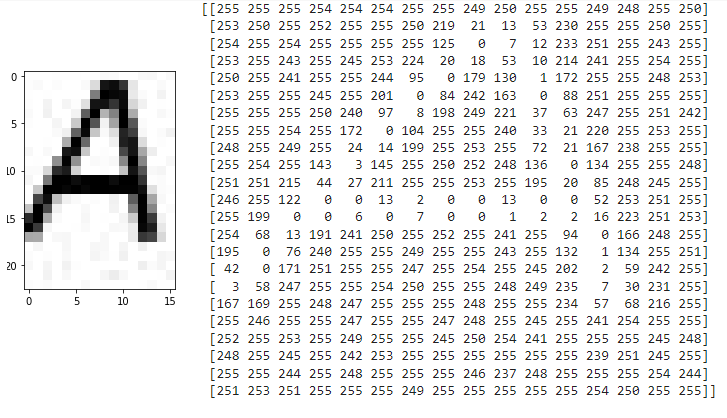
\includegraphics[width=0.7\textwidth]{annexes/img/A_to_matrix.png}
	    \caption{Transposition d'un caractère en matrice (niveau de gris)}
	    \label{fig:a_matrix}
	\end{figure}
	
	Cette transposition de l'image en une matrice décimale facilite la détermination d'un caractère \textit{via} l'application de modèles statistiques et mathématiques. L'une des premières méthodes appliquées dans le domaine de l'apprentissage machine est la méthode \textit{k-NN}(Méthode des k plus proches voisins)\footcite[p.~39]{terrielRepresenterEvaluerDonnees2020}. Pour la définir, cette technique d'apprentissage supervisée réside sur l'alignement de données étiquetées, en établissant la donnée équivalente la plus proche (la distance \textit{k}) de notre caractère x. À partir des années 1980, les laboratoires travaillant sur la reconnaissance d'écriture réutilisent les avancées dans le domaine de la linguistique et de ses modèles arithmétiques (\textit{Hidden Markov Model}) s'appuyant sur des systèmes d'occurrences et de nouveaux modèles de segmentation\footcite[p.~40]{terrielRepresenterEvaluerDonnees2020}.
	
	\subsubsection{\textit{Reconnaissance de texte et apprentissage profond}}
	
	De nos jours, les techniques de reconnaissance de texte se sont considérablement améliorées. Ce perfectionnement est dû à l’explosion du \textit{deep learning} (apprentissage profond) en 2012, suite à la victoire incontestable d'un de ces modèles lors d'un concours de classification d'images. Le procédé n'est pas nouveau puisqu'on peut remonter son origine à 1943, où le neurologue et le logicien Warren S. McCulloch et Walter Pitts décrivent une première application \enquote{neuronale} de la machine de Turing\footcite{mccullochLogicalCalculusIdeas1943}. Toutefois, la parenté de l'apprentissage profond est encore contestée puisque le chercheur Charles C. Tappert rattache davantage sa première conceptualisation à Frank Rosenblatt et son invention du perceptron\footcite[Il met en place un système probabiliste de stockage et de classifications de l'information s'appuyant sur le modèle d'un réseau neuronal][]{tappertWhoFatherDeep2019}.
	
	Le \textit{deep learning} reste en marge au sein de l'intelligence artificielle pendant de nombreuses années en raison de la puissance de calcul nécessaire à son fonctionnement intrinsèque. Malgré tout, certaines équipes de chercheurs comme celle dirigée par Yann Le Cun continuent de développer la recherche fondamentale, permettant en 2012 d'exploser les records aux yeux du monde.
	
	\begin{figure}[h!]
	    \centering
	    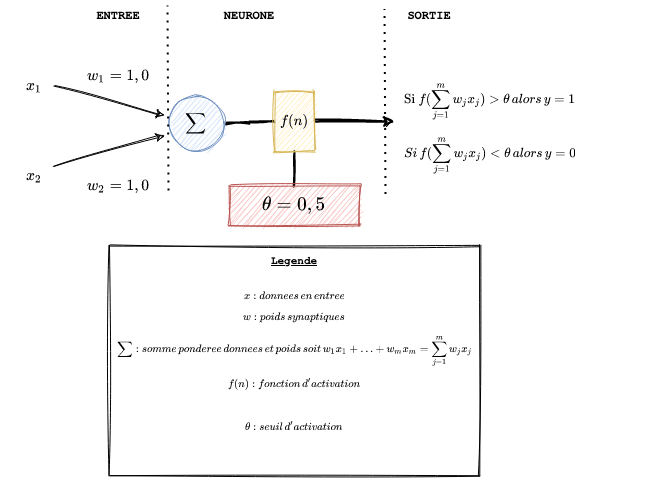
\includegraphics[width=0.9\textwidth]{annexes/graph/neurone_formel.png}
	    \caption{Illustration simplifiée d’un neurone formel, ©Lucas Terriel, 2020}
	    \label{fig:neurone}
	\end{figure}
	
	L'apprentissage profond se veut donc à la frontière de l'informatique, des mathématiques et de la neurobiologie en reprenant le modèle du neurone et du système de stimulation synaptique. Cette artificialisation numérique s'appelle le perceptron \textit{alias} le neurone simple. Pour reprendre la métaphore, le neurone reçoit une quantité d'information (les poids) dont la somme pondérée doit atteindre un certain seuil afin d'être stimulée. Cette stimulation applique une fonction d'activation ou de transfert envoyant une information de sortie (voir figure \ref{fig:neurone}). À partir de ce système, des réseaux de neurones sont alors mis en place afin de traiter des données complexes, et ce avec une spécialisation progressive. De nos jours, l'algorithme du perceptron simple est dépassé au profit de systèmes améliorés tel que le perceptron multicouche, consistant en une série de neurones simples et cachés, ou le \textit{Support Vector Machine}\footcite[Pour prolonger la curiosité, voici trois articles permettant d'expliquer certains principes généraux et des cas applicatifs:][]{nobleWhatSupportVector2006, gardnerArtificialNeuralNetworks1998, ramchounMultilayerPerceptronArchitecture2016}.
	
	À l'image de l'ensemble du domaine de l'intelligence artificielle, l'apprentissage profond a connu une véritable ébullition dans le secteur de la reconnaissance automatique de texte, et ce particulièrement après 2016\footcite{memonHandwrittenOpticalCharacter2020}. Les résultats furent rapidement très satisfaisants grâce à la capacité des réseaux de neurones à traiter des données complexes et en sa capacité de mémorisation. C'est justement sur ce dernier point que certains laboratoires ce sont appuyés pour améliorer les résultats concernant les écritures manuscrites en incitant l'utilisation d'une architecture \gls{RNN}. Cette architecture traite l'information de manière cyclique et lui permet donc de la contextualiser. Elle a rapidement affiché des taux supérieurs à 90\%, néanmoins au détriment d'une très imposante puissance de calcul\footcite{gravesOfflineHandwritingRecognition2008}. Cette architecture reste encore aujourd'hui la plus commune, même si régulièrement présente sous forme hybride. Toutefois, plusieurs groupes de chercheurs ont signalé les problèmes sous-jacents de cette architecture à la fois sur le plan technique (la distorsion et l'explosion des très grandes images) et les besoins exponentiels en terme de puissance de calcul. Les systèmes hybrides couplés avec les architectures \gls{CNN} semblent remettre en cause la suprématie des réseaux RNN en permettant une réduction considérable du coût de calcul grâce à un système de segmentation des tâches, accentué par un traitement de l'image plus important (notamment le processus d'augmentation)\footcite{puigcerverAreMultidimensionalRecurrent2017, desousanetoHTRFlorDeepLearning2020}.
	
	\subsection{La révolution technique de l'\gls{htr}}
	
	Comme nous l'avons vu précédemment, le \textit{deep learning} a consolidé amplement les nombreuses avancées dans la reconnaissance de texte et plus particulièrement le secteur de l'\gls{htr}. Dans la majorité des projets, les techniques d'apprentissage se fondent sur l'apprentissage supervisé. C'est-à-dire qu'on fournit au processus d'apprentissage des données préalablement étiquetées afin de lui fournir un support d'apprentissage à partir duquel la machine va pouvoir déployer une méthode d'analyse, et ainsi classifier les caractères.
	
	Néanmoins, la \gls{rem} n'est pas simplement due à l'essor de l'apprentissage profond, même si les avancées techniques lui sont que corrélées. En effet, l'\gls{htr} correspond à un procédé de segmentation bien spécifique en comparaison des techniques portant sur l'\gls{ocr}. Le point névralgique de cette technique de reconnaissance de texte réside dans la segmentation de l'image dans son intégralité, et non sur un centrage spécifique. À l’origine, le moteur établit un masque définissant la zone à reconnaître à partir d'une ligne de référence, souvent en bas\footcite[p.~25-26]{noemieOCRHTRGraphie2022}. Ce point d'appui permet d'exercer ce que l'on appelle la reconnaissance en-ligne ce qui signifie une conception des caractères cursifs dans l'espace et le temps par la machine. Le modèle, s'appuyant sur son expérience, va donc déchiffrer l'écriture selon ses mouvements et les comparer aux données terrain. D'autres méthodes tendent à remplacer le procédé par ligne par un système à polygone (\textit{bounding boxes}) depuis quelques années à l'image des groupes de chercheurs de l'\gls{ephe} ou de l'Université autonome de Barcelone\footcite{carbonellNeuralModelText2020, kiesslingBADAMPublicDataset2019}. Comme l'expose la figure \ref{fig:mask_baseline} s'appuyant sur le moteur kraken développé par l'\gls{ephe}, la reconnaissance des caractères s'appuie sur la détection de ligne afin de délimiter une zone de contour, un polygone permettant une meilleure détection et évaluation de l'objet\footcite[p.~26]{noemieOCRHTRGraphie2022}.
	
	\begin{figure}[h!]
	    \centering
	    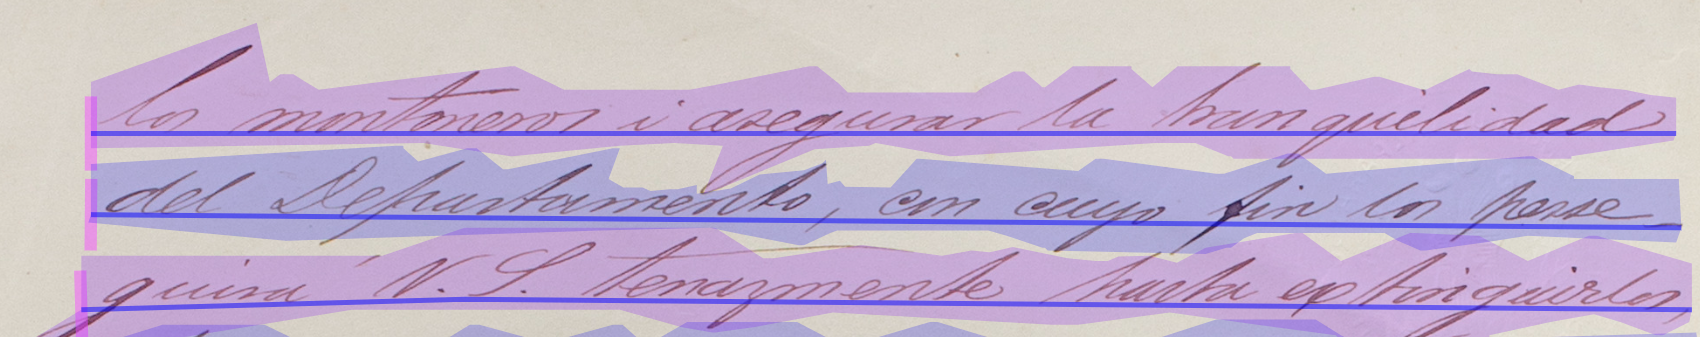
\includegraphics[width=1\textwidth]{annexes/img/mask_baseline.png}
	    \caption{Exemple de masque à partir d'une \textit{baseline}}
	    \label{fig:mask_baseline}
	\end{figure}
	
	La reconnaissance de texte n'est donc qu'une étape au sein d'un moteur \gls{htr}. Si l'on regarde le schéma suivant (figure \ref{fig:htr_schema}), on remarque trois étapes primordiales à l'obtention d'une prédiction qualitative. La détermination de cette chaîne de traitement a caractérisé de nombreux progrès au sein de la \gls{rem} et plus particulièrement au sein des écritures complexes usant de nombreux glyphes tel que l'arabe\footcite{kiesslingBADAMPublicDataset2019}. En outre, une phase de traitement des données de sorties est régulièrement ajoutée au sein des projets afin de maximiser les résultats.
	
	\begin{figure}[h!]
	    \centering
	    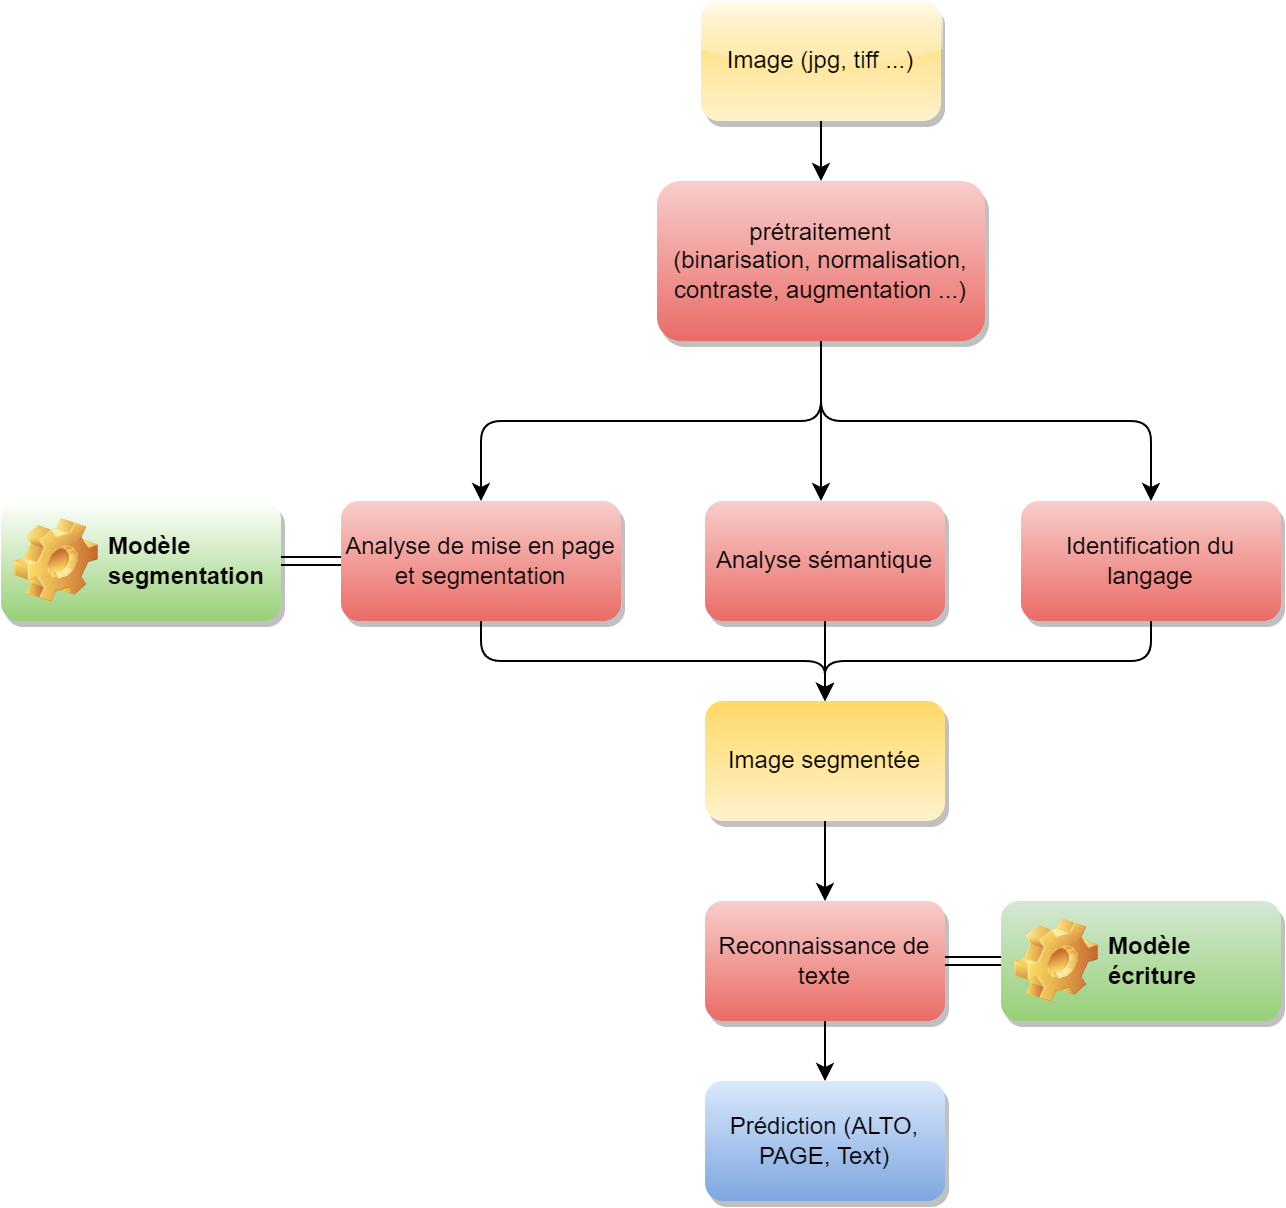
\includegraphics[width=1\textwidth]{annexes/schema/HTR_processus.png}
	    \caption{Chaîne de traitement d'un procédé \gls{htr}}
	    \label{fig:htr_schema}
	\end{figure}
	
	\subsection{\texttt{Kraken} et \texttt{eScriptorium}: moteur et application pour l'HTR}
	
	Avec l'explosion du \textit{deep learning} et de l'\gls{htr}, de nombreuses plateformes dédiées ont fait leur apparition au sein de la sphère de la \gls{rem}. Une en particulièr s'est rapidement imposée de part la qualité de ses résultats: \textit{Transkribus}, avec le financement du projet européen READ-IT(Reading Europe Advanced Investigation Tools). Elle propose des modèles extrêmement complets, permettant d'obtenir des résultats très qualitatifs. Originalement gratuite, son utilisation est devenue payante au fil du temps, tournant de nombreux projets d'édition numérique vers d'autres outils \textit{open source} tel qu'\gls{eScriptorium}.
	
	L'initiative du projet est née en 2019 par un groupe de chercheurs issus de l'institut de recherche Scripta de l'écosystème Paris Science et Lettres, et plus particulièrement de l'\gls{ephe}. Le but est de fournir une interface web de \gls{rem} à destination de l'histoire scientifique et la plus ouverte possible, en réaction à l'opacité du projet Transkribus et son nouveau modèle économique\footcite{kiesslingEScriptoriumOpenSource2019}. Le second objectif est de renforcer la \gls{rem} sur un panel de langages beaucoup plus importants grâce au soutien des compétences du laboratoire. Ce besoin naît du constat que les principaux modèles sont essentiellement adaptés aux langues latines. Scripta doit permettre d'étendre le fonctionnement de la \gls{rem} à des langues et des documents plus complexes comme le signale Peter A. Stokes:
	
	\begin{quote}
	    \enquote{It has therefore been a crucial element of the project that the software must avoid, as far as possible, all assumptions about the nature of the writing and language that is in the system. The writing may be left to right, right to left, top to bottom or even bottom to top; the support may be paper, parchment, but also stone, palm leaf, clay, wood, or many others; it may be written with a pen, painted with a brush, inscribed with a chisel; the writing system may be alphabetic, logographic, hieroglyphic; and so on.\footnote{\enquote{Un élément crucial du projet a donc été que le logiciel doit éviter, autant que possible, toute hypothèse sur la nature de l'écriture et de la langue qui se trouve dans le système. L'écriture peut être de gauche à droite, de droite à gauche, de haut en bas ou même de bas en haut ; le support peut être du papier, du parchemin, mais aussi de la pierre, de la feuille de palmier, de l'argile, du bois, ou bien d'autres encore ; elle peut être écrite à la plume, peinte au pinceau, inscrite au ciseau ; le système d'écriture peut être alphabétique, logographique, hiéroglyphique ; et ainsi de suite.} \textit{in} \cite{stokesEScriptoriumVREManuscript}}}
	\end{quote}
	
	La plateforme \gls{eScriptorium} s'appuie sur le moteur \gls{ocr} \gls{kraken} développé par Benjamin Kiessling. \gls{kraken} est un moteur clé en main interactif sous la forme d'un \gls{cli}, optimisé pour les documents historiques et les textes en caractères non latins\footcite{kiesslingKrakenUniversalText2019a}. Basé sur le moteur Ocropy, \gls{kraken} offre une très grande modularité lors de la conception de modèle de segmentation ou de reconnaissance de texte, mais aussi de multiples schémas de sortie ce qui en fait un moteur rapidement intégral au sein d'une chaîne de traitement. Le moteur est construit sur deux architectures neuronales différentes. À l’origine, le système de détection des \textit{baselines} utilise une architecture mixte \gls{CNN} et LSTM (\textit{long short-term memory}) qui est une catégorie des modèles \gls{RNN}\footcite{toselliDigitalEditionsDistant2021a}. Plusieurs études ont démontrée la capacité de cette architecture neuronale mixte à limiter le nombre de vérités terrain nécessaires à la production d'un modèle\footcite{aradillasBoostingHandwritingText2018, granetTransferLearningHandwriting2018}. Ces expérimentations architecturales et ces observations empiriques ont permises une réelle amélioration de la \gls{rem}.
	
	\begin{figure}[h!]
	    \centering
	    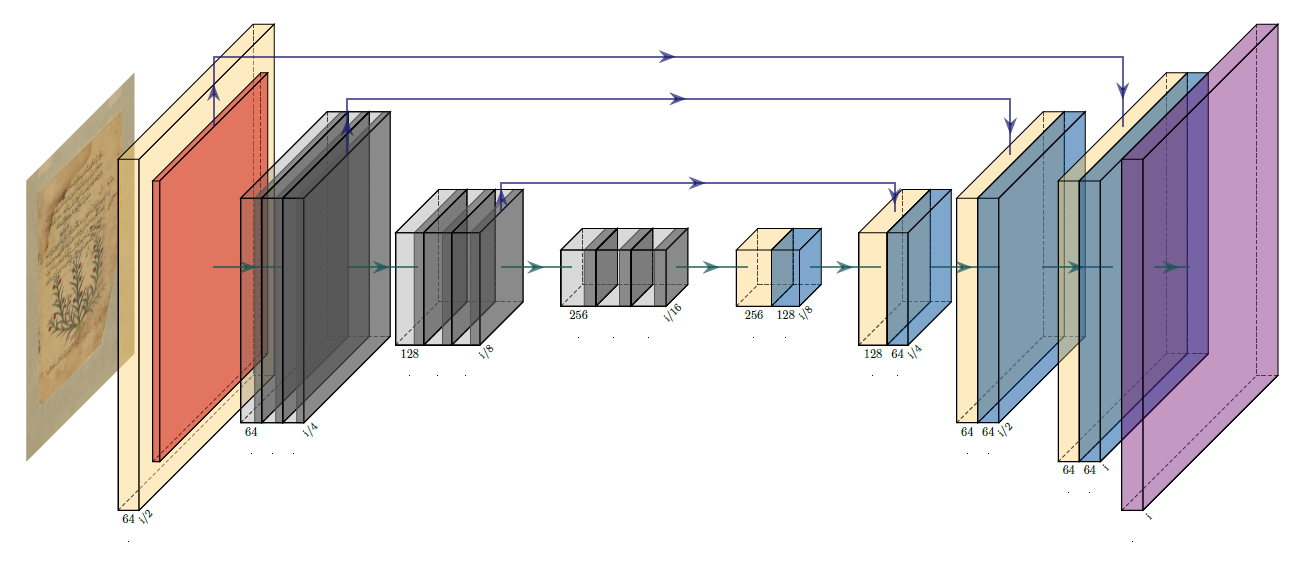
\includegraphics[width=0.8\textwidth]{annexes/schema/CNN_network.png}
	    \caption{Architecture \gls{CNN} à échantillonnage et BLSTM de détection des \textit{baselines} au sein du moteur Kraken - @Benjamin Kiessling, 2019}
	    \label{fig:cnn_archi}
	\end{figure}
	
	
	\section{Méthodologie appliquée à la production d'un modèle HTR}
	
	La plateforme \gls{eScriptorium} et le moteur \gls{kraken} ont été au centre du processus de transposition numérique des données autour des archives de l'Occupation de l'Araucania. La volonté initiale d'orienter son moteur vers le traitement des documents historiques ouvre ainsi de multiples possibilités pour la production d'une chaîne de traitement dédiée à l'édition numérique historique. En outre, le choix de procéder à une application ouverte, gratuite et modulable renforce l"accessibilité de cette technologie à des projets plus modestes et expérimentaux.
	Dans ce cadre, nous allons observer comment a été conçu à modèle \gls{rem} adapté à ces archives à partir du moteur \gls{kraken}.
	
	\subsection{Produire un modèle \gls{htr} avec \gls{kraken}}
	
	Initialement le projet souhaitait s'appuyer directement sur les ressources \textit{hardware} de la plateforme \gls{eScriptorium}, car comme nous l'avons vu le moteur \gls{kraken} nécessite une très forte puissance de calcul en raison de son architecture neuronale \gls{RNN}. Toutefois, cette puissance exigée a aussi un coût pour la structure de l'\gls{inria} et le temps d'attentes peut être assez long en fonction de la demande. Il a donc rapidement été décidé de passer par des moyens alternatifs en s'appuyant sur un \gls{gpu} personnel et d'utiliser directement le \gls{cli} \gls{kraken}.
	
	Pour la méthodologie employée, il convient de définir quelques termes complexes. Le processus d'apprentissage supervisé s'appuie sur trois types de données qui ont été préalablement compilées afin d'améliorer les performances : les données d'entraînements, les données de validation qui vont être le support d'apprentissage lors de l'entraînement et enfin les données de tests qui vont permettre d'évaluer la qualité de l'apprentissage. En général et ici dans notre cas, les données sont réparties entre 80\% pour les données d'entraînements, 10\% pour les données de validation et 10\% pour les données de tests. Chaque processus d'entraînement est nommé \textit{epoch} et se termine par la procédure d'évaluation. Lors de chaque entraînement, les données sont subdivisées en différents lots d'apprentissage simultané (\textit{batch}) permettant d'améliorer la qualité d'analyse du modèle\footcite[Pour plus de détails, la documentation de Kraken est particulièrement explicite dans le fonctionnement de l'apprentissage \textit{in}]{kiesslingKrakenOCRSystem2022}. La fin générale du processus d'entraînement s'applique selon plusieurs critères. Une limite s'applique quand s'effectue une normalisation des scores et ainsi éviter le risque d'\textit{overfitting}. Il s'agit d'un risque de surspécialisation du modèle qui tend à apprendre les données "par coeur". Il devient ainsi incapable d'agir correctement face à de nouvelles données.
	
	\begin{figure}[h]
	    \centering
	    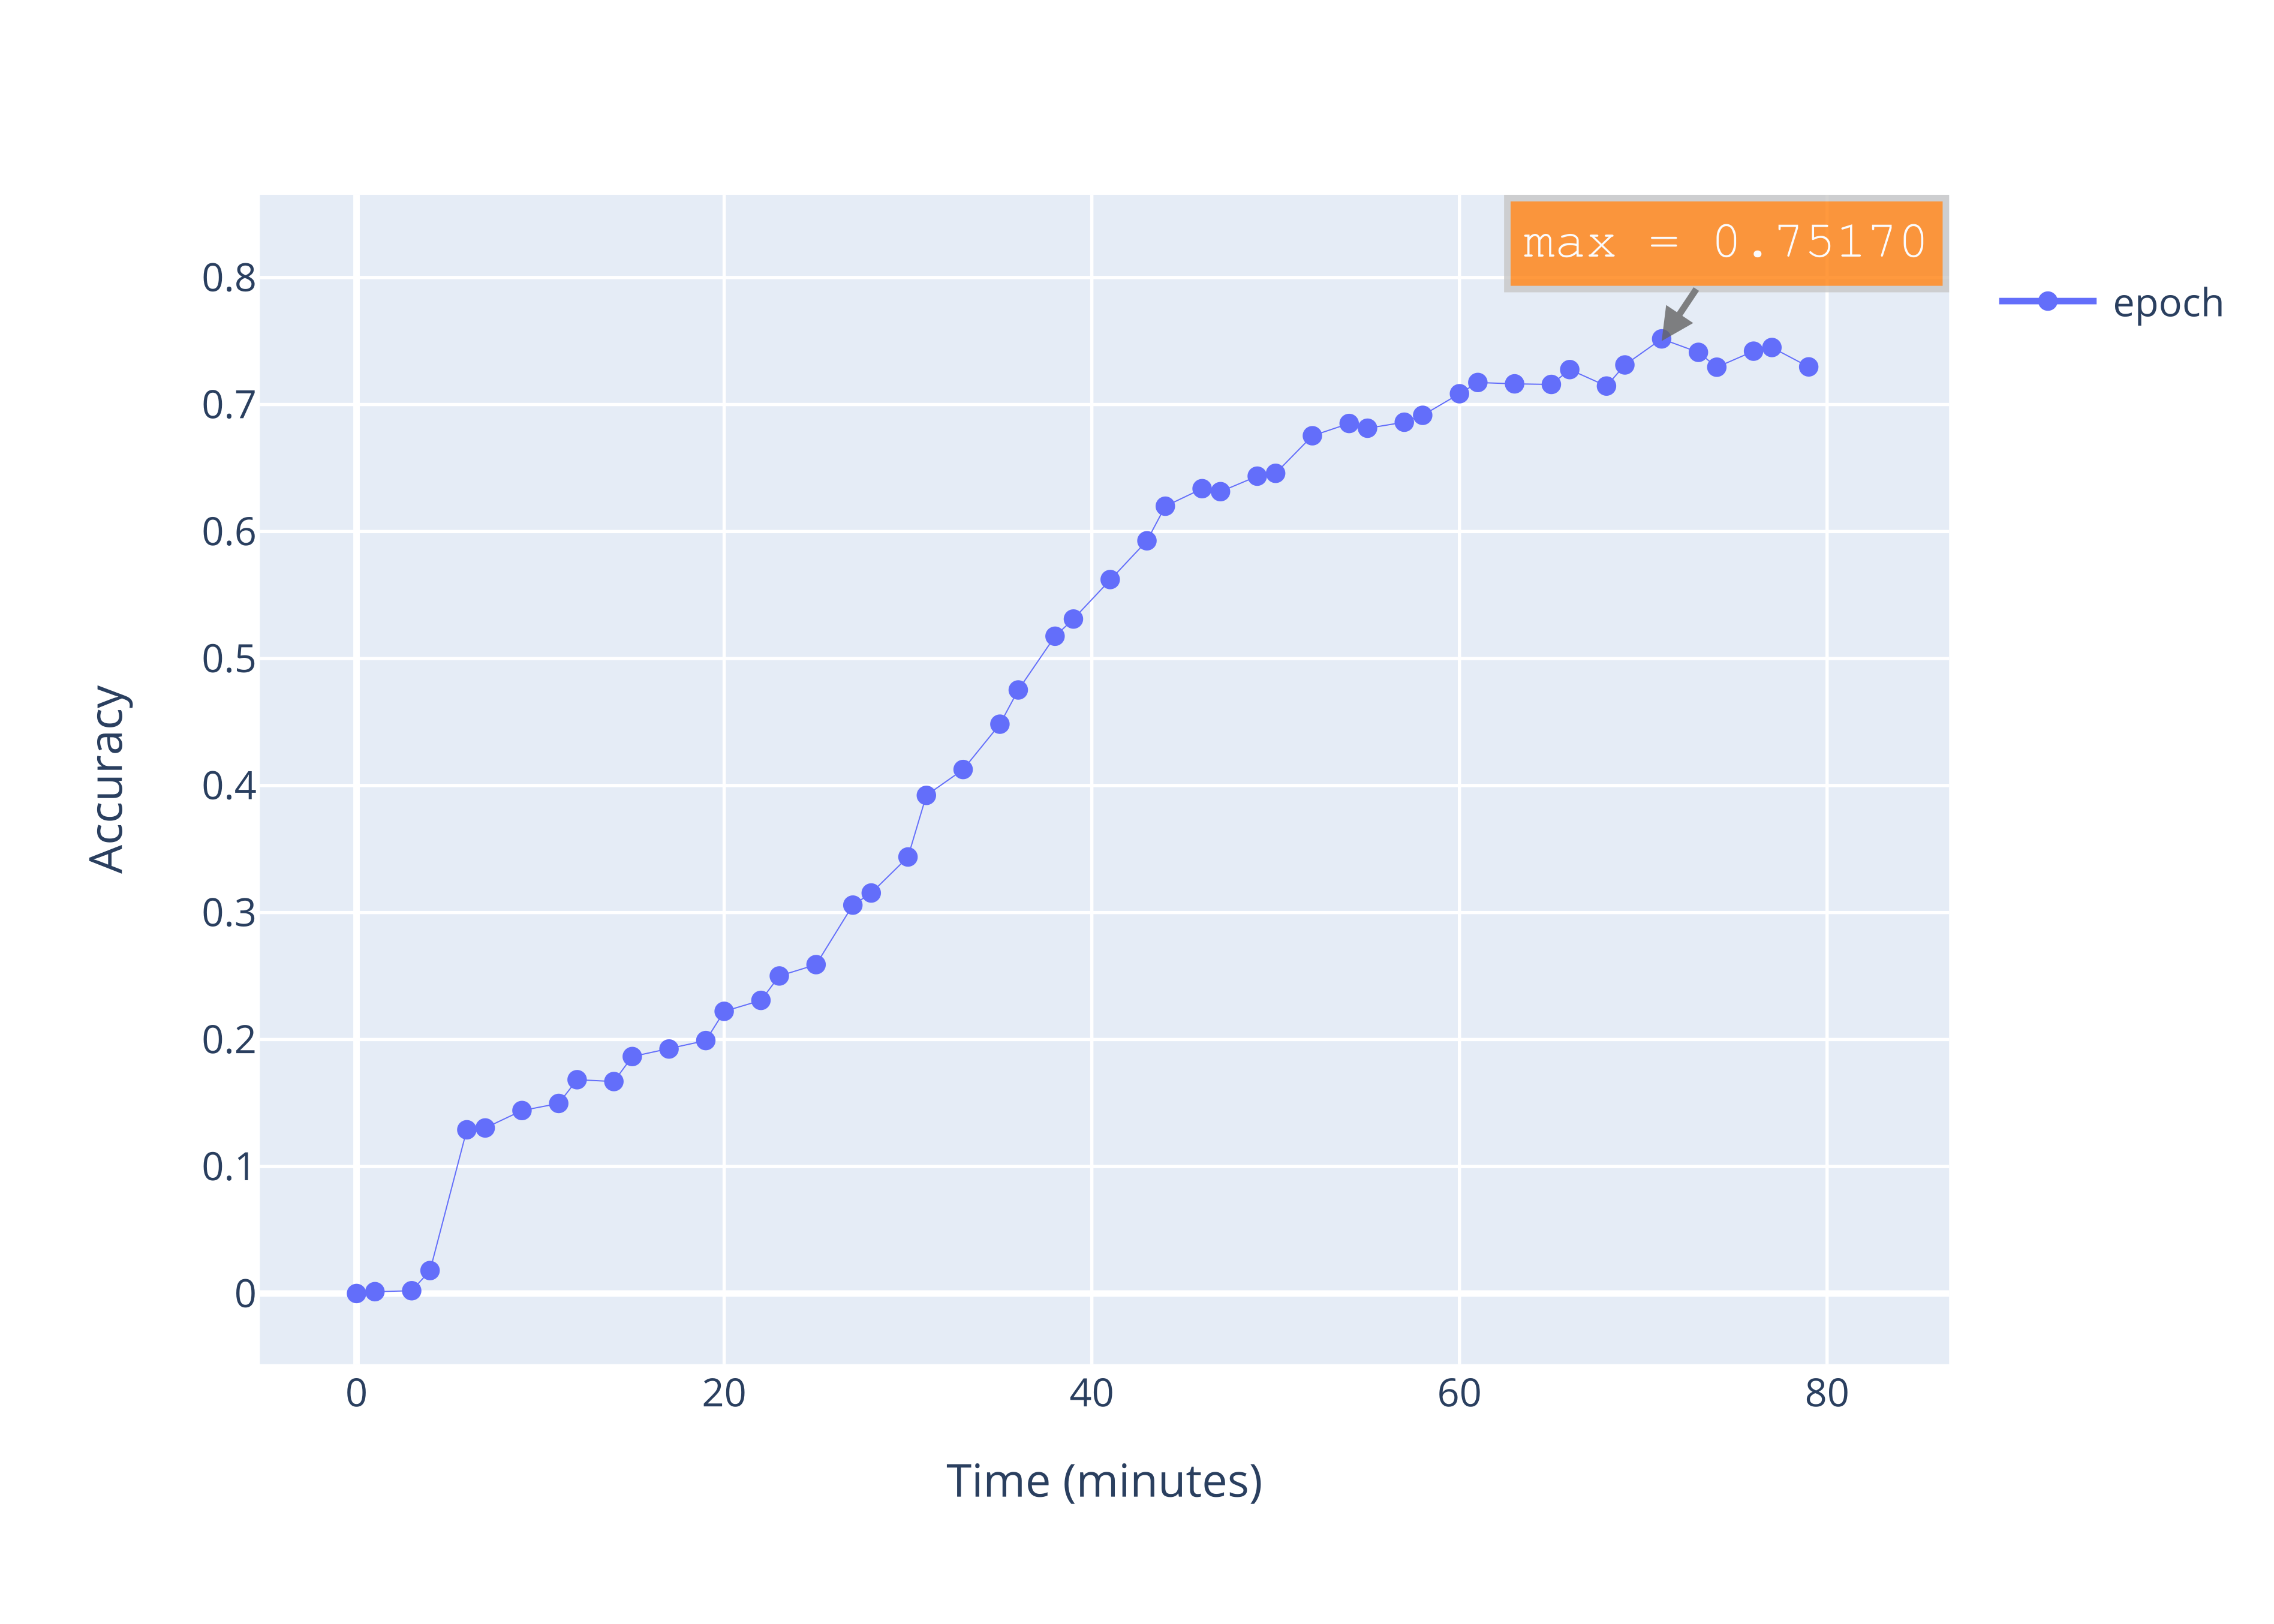
\includegraphics[width=1.1\textwidth]{annexes/graph/train_epoch.png}
	    \caption{Entraînement d'un modèle avec la méthode \textit{skratch}}
	    \label{fig:epoch_skratch}
	\end{figure}
	
	Le moteur développé par Benjamin Kiessling permet de créer son modèle à partir de deux méthodes de \textit{machine learning} : le modèle \textit{skratch} dont les données d'apprentissages sont natives ce qui signifie un apprentissage \textit{ad hoc}, et la technique du \textit{transfert learning} qui correspond à la réutilisation d'un modèle pré-entrainé et d'en exploiter les connaissances basiques en reprenant son architecture et en y ajoutant des données \textit{ad hoc}. L'entraînement \textit{via fine-tuning} est donc une sous catégorie du \textit{transfert learning}, assez propre aux architectures \gls{CNN}, puisque cette méthode permet de réadapter les poids neuronaux au cours de l'apprentissage ce qui conduit à affiner le modèle. Il faut penser qu'au sein du réseau neuronal, les neurones situés en premières séries ont très souvent des tâches génériques alors que les dernières séries de neurones ont la plus grande part une fonction très spécifique. Tout l'enjeu de ce procédé est finalement d'affiner les poids de ces derniers.
	
	Les avantages du \textit{transfert learning} puisqu'il est désormais possible de produire des modèles performants à moindre coût, en limitant le besoin de produire des données terrains\footcite{aradillasBoostingHandwritingText2018}. Coupler les données en puisant sur des neurones existants permet généralement d'obtenir de très bon, voir d'excellents résultat. Vincent Jolivet estime aujourd'hui que le fine-tuning est devenu la norme au sein du paysage de la \gls{rem}, en permettant de créer des modèles à moindre coût \footcite{torresHTRFineTuning2022}. La multiplication des plateformes de partage de données et de modèles est ainsi indispensable au développement de cette stratégie, et \textit{de facto} à la démocratisation de l'\gls{htr}.
	
	\subsection{Modélisation, résultats et interprétations}
	
	Afin d'observer concrètement les avantages et les inconvénients de ces deux méthodes, plusieurs modèles ont été réalisés afin de déterminer le réseau neuronal le plus performant pour déchiffrer des sources manuscrites de multiples mains\footnote{Les lignes de commandes utilisées avec le moteur kraken sont observables en annexe (voir figure \ref{code:skratch} et \ref{code:finetuning}}).
	
	\subsubsection{\textit{Datasets} et modèles}
	
	En plus des données produites, deux jeux de données extérieurs ont été utilisés : les archives notariales du projet \gls{lectaurep} et le modèle éponyme, ainsi que les archives des testaments de poilus\footcite{durandNotairesParisRepertoires2021, clericeCREMMAANTestamentDePoilus2022}. Ces deux \textit{datasets} peuvent être rapprochés de nos données terrains, car ils sont composés de documents avec une écriture cursive contemporaine (XIX\textsuperscript{e} siècle). 
	
	La difficulté consiste à disposer de suffisamment de données terrains propres afin de \enquote{casser le modèle de langue}, car on le rappelle, les moteurs \gls{htr} s'appuient sur le traitement du langage pour affiner ces prédictions. Enfin, nous nous sommes fondés sur le récent méga-modèle \textit{Manu MacFrench} développé par Thibault Clérice et Alix Chagué\footcite{chagueHTRUnitedManuMcFrench2022}.
	
	
	\subsubsection{Résultats et analyses}
	
	\begin{table}
    \centering
    \resizebox{\textwidth}{!}{%
    \begin{tabular}{|l|l|l|l|l|l|}
    \hline
    \multicolumn{1}{|c|}{\textbf{Name}} & \multicolumn{1}{c|}{\textbf{Quantity (GT)}} & \multicolumn{1}{c|}{\textbf{Val\_acc}} & \multicolumn{1}{c|}{\textbf{Test\_acc}} & \multicolumn{1}{c|}{\textbf{CER}} & \multicolumn{1}{c|}{\textbf{WER}} \\ \hline
    ArSKR                               & 180                                         & 0.75170                                & 0.77860                                      & 0.26558                                & 0.38640                                \\ \hline
    ArLCTP                              & 144                                         & 0.93328                                & 0.83570                                      & 0.04410                                & 0.18993                                \\ \hline
    ArLCTP-NFKD                         & 144                                         & 0.91871                                & 0.84650                                      & 0.03668                                & 0.15853                                \\ \hline
    ArLCTP+pl                           & 244                                         & 0.91697                                & 0.83230                                      & 0.05045                                & 0.21338                                \\ \hline
    ArMcFR                              & 180                                         & 0.90354                                & 0.86730                                 & 0.05598                                & 0.21423                                \\ \hline
    ArMcFR-NFKD                         & 180                                         & 0.89872                                & 0.85630                                      & 0.06646                                & 0.24963                                \\ \hline
    \end{tabular}%
    }
    \caption{Résultats des modèles HTR\protect\footnotemark}
    \label{tab:results_htr}
    \end{table}
    
    \footnotetext{ArSKR : modèle \textit{skratch dataset ad hoc}; ArLCTP : \textit{fine-tuning} avec modèle \gls{lectaurep}; ArLCTP+pl : \textit{fine-tuning} avec modèle \gls{lectaurep} et ajout du jeu de données des testaments de poilus; ArMcFR : \textit{fine-tuning} avec modèle \textit{Manu MacFrench}.}
    
    Comme nous pouvons le constater au sein du tableau \ref{tab:results_htr}, les différentes méthodes employées ont affichés des résultats assez contrastés. La valeur \gls{ACC} proposée par kraken lors du processus d'entraînement a rapidement été insuffisante pour comparer et optimiser le caractère. Lors de la compilation préalable des fichiers, la désignation des fichiers tests est donc hasardeuse et les résultats obtenus sont alors intrinsèquement relatifs. Dans un premier temps, nous nous sommes appuyés sur l'application \texttt{KaMi-Lib} développée par l'\gls{inria} et plus particulièrement Lucas Terriel\footcite{terrielKaMIlib2022}. Elle permet d'étendre le nombre de mesures possibles afin d'étudier plus en profondeur les prédictions \gls{ocr} en fonction des vérités terrains, mais aussi d'obtenir certains mesures relevant du \gls{tal}. Au sein de chaque main principale, un échantillon a été prélevé afin de constituer les données de terrains de l'évaluation par \texttt{KaMi-Lib}\footcite{humeauHTREvaluation2022}. Les principales mesures qui ont été utilisées pour comprendre l'efficacité des modèles \gls{rem} sont les métriques \gls{CER} et \gls{WER}, permettant de donner le taux d'erreurs par caractères et par mots. En parallèle, un jeu de données tests a été constitué afin de déterminer le taux \gls{ACC} à partir d'une main inconnue et de qualité moyenne. 
    
    À première vue, le modèle ArLCTP, \textit{fine-tuned} à partir du modèle déployé par le projet \gls{lectaurep}, semble donner les meilleurs résultats. En revanche, en le comparant aux données issues de l'évaluation test, le taux \gls{ACC} est bien plus faible, laissant penser à un possible phénomène d'\textit{overfitting} en raison de sa mauvaise adaptation. Le modèle ArMcFR semble ainsi offrir les résultats les plus polyvalents et indiquant une meilleure performance malgré des taux \gls{CER} et \gls{WER} légèrement plus élevés. Il reste tout de même perfectible en vue de ces résultats pouvant être qualifiés de \enquote{moyen-bon} en raison de ses taux d'erreurs\footcite[Dans cette article, il est estimé que le \gls{CER} doit être inférieur à 2 afin d'être qualifié de très bon voir d'excellent]{tomoiagaFieldTypingImproved2019}. Lors du colloque \enquote{Documents anciens et reconnaissance automatique des écritures manuscrites} qui se déroulait en juin 2022, Vincent Jolivet et Sergio Torres ont estimé qu'un taux \gls{ACC} de 90\% doit être comme considéré comme le seuil sur l'échelle du rapport coût de production et efficacité du modèle\footcite{torresHTRFineTuning2022}. De même, Maciej Eder estime que le bruit des données au sein des corpus textuels n'affecte pas singulièrement les recherches autour, la stylométrie dans ce cas précis, si le taux de corruption des données est inférieur à 20\%\footcite{ederMindYourCorpus2013}.
    
    Toutefois, il reste à évaluer la capacité du modèle à être affiné selon les situations. Sans avoir pu être réalisée en l'état, l'agrégation de quelques nouvelles données terrains sur une main bien particulière pourrait permettre d'atteindre des taux extrêmement satisfaisants comme le souligna Ariane Pinche au cours de ce même colloque\footcite{pincheSegmOntoControlledVocabulary2022a}.
	
	\subsubsection{Difficultés et encodage}
	
	En reprenant le tableau \ref{tab:results_htr}, on peut constater la présence de modèles NFKD (\textit{Normalization Form Canonical Decomposition}). Il s'agit d'un système d'uniformisation au sein des caractères Unicode. La méthode NFKD permet dans ce cas de décomposer les caractères diacritiques, en un ensemble de caractères Unicode permettant une appréhension fondamentale, en conservant sa relation canonique et ordonnée. Les divers essais montrent une appropriation relative des modèles \gls{htr} à cette uniformisation. On remarque au sein du tableau \ref{tab:error_htr} que la gestion des accents représente le sixième type d'erreurs les plus fréquentes.
	
	\begin{table}
    \centering
    \resizebox{0.4\textwidth}{!}{%
    \begin{tabular}{|c|c|c|}
    \hline
    \textbf{Nombre} & \textbf{Correct} & \textbf{Généré} \\ \hline
    40              & s                & c               \\ \hline
    24              & SPACE            & NONE            \\ \hline
    22              & i                & e               \\ \hline
    21              & o                & a               \\ \hline
    21              & r                & s               \\ \hline
    20              & ACCENT           & NONE            \\ \hline
    18              & s                & r               \\ \hline
    \end{tabular}%
    }
    \caption{Les 7 erreurs les plus courantes du modèle ArMcFR}
    \label{tab:error_htr}
    \end{table}
    
    En examinant plus attentivement les erreurs récurrentes du modèle, on peut rapidement identifier plusieurs lacunes et confusions, en particulier la reconnaissance des caractères Unicode 'r' et 's'. Cette répétitivité amène à un \gls{WER} moyen indiquant un mot erroné tous les cinq mots. Ces confusions peuvent s'expliquer par la fréquence élevée de ces caractères au sein de la langue espagnole et de la proximité graphologique entre les caractères. 
    
    \begin{figure}
        \centering
        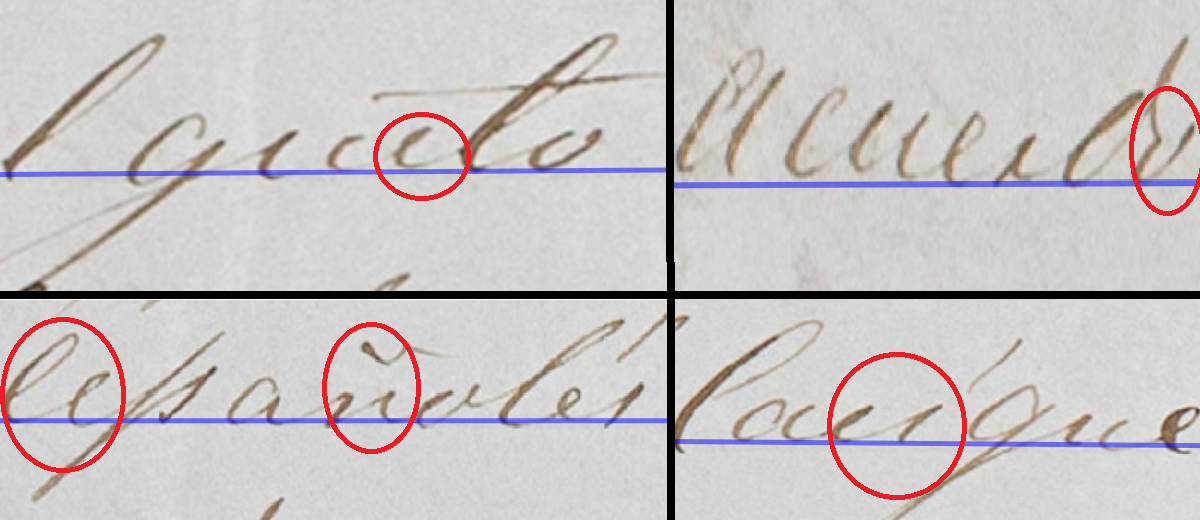
\includegraphics[width=0.9\textwidth]{annexes/img/error_HTR.png}
        \caption{Exemple d'erreurs courantes pour le modèle ArMcFR\protect\footnotemark}
        \label{fig:error_htr}
    \end{figure}
    
    \footnotetext{Image haut gauche : guito/ gusto; image haut droite: acuerd/acuerdo; image bas gauche: lepanoles/españoles; image bas droite: Caesque/Cacique.}

    
    En observant plus en détail, la distance des mots, selon l'algorithme de distance de Levenshtein, se situe autour d'une moyenne tronquée autour de 43, mais avec un écart-type plus conséquent concernant les mains Villalon et Saavedra. Cette distance semble \textit{a priori} suffisamment faible indiquant une relative concordance entre les mots prédits et les mots corrects, limitant le risque d'altérer le sens initial\footcite{terrielAtelierProductionModele2021}. À partir de cette distance, Thi-Tuyet-Hai Nguyen et al. classe deux types d'erreurs : les erreurs simples et les erreurs complexes ayant un nombre d'erreurs supérieur à 1\footcite{nguyenDeepStatisticalAnalysis2019}. Ces erreurs vont plus ou moins être influencées selon la longueur des mots et la gestion des espacements des modèles \gls{ocr} et ainsi augmenter le risque de cette distance.
    
    Il est donc toujours difficile d'évaluer correctement un modèle, et plus encore, de sélectionner le modèle le plus performant dans le cadre d'une application contrainte et spécifique. Dans notre cas, nous sommes appuyés sur des métriques basées sur le lexique dont le modèle ArMcFR semble ressortir comme le plus complet. Cependant, à l'heure de la massification des solutions \gls{tal} certaines mesures pourraient reprendre les évaluations par système de masque sur le modèle des architectures encodeurs-décodeurs comme le constatent Phillip Benjamin Strobel et al.\footcite{strobelEvaluationHTRModels2022}.
    
    \begin{figure}[H]
	    \centering
	    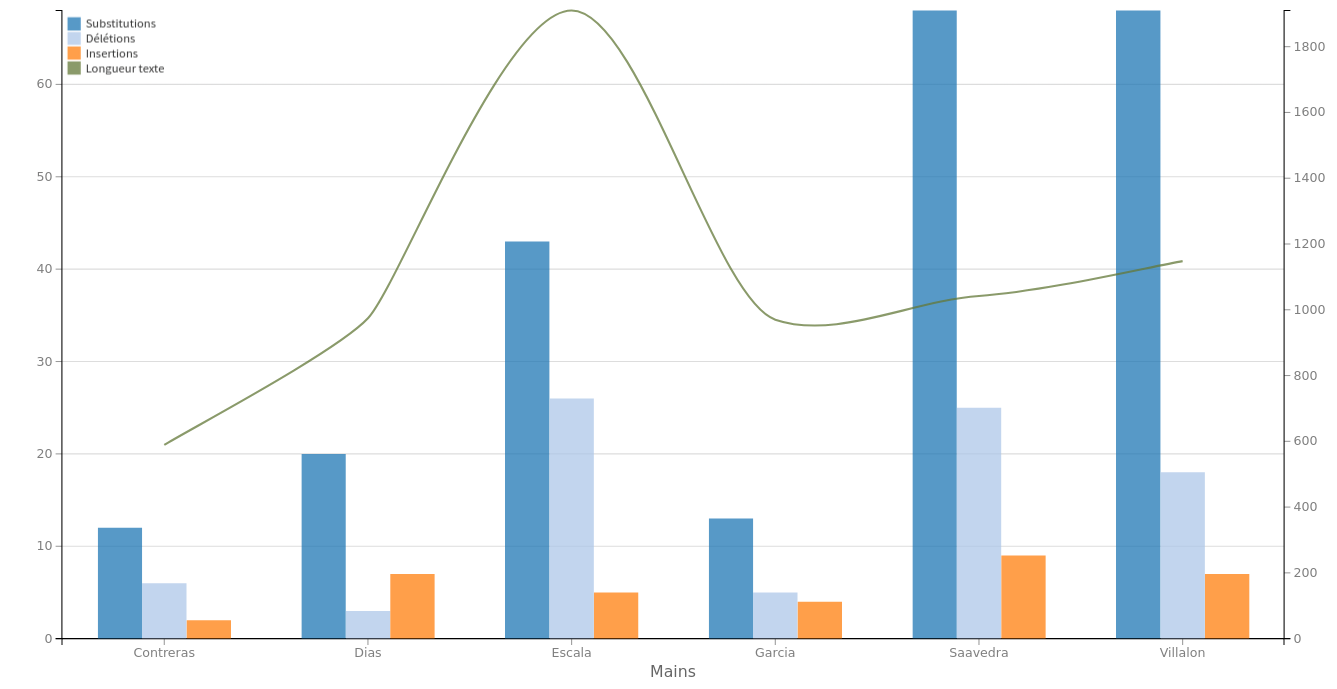
\includegraphics[width=0.9\textwidth]{annexes/graph/DIS_htr.png}
	    \caption{Évaluation \gls{DIS} du modèle ArMcFR avec \texttt{KaMi-Lib}}
	    \label{fig:dis_htr}
	\end{figure}
	
	
	\subsection{Les difficultés d'un modèle de segmentation}
	
	À partir de notre lot de transcriptions, nous avons dans le même temps essayer de produire un modèle de segmentation \gls{htr} à partir du moteur \gls{kraken}. Il fait suite à la volonté d'automatiser la segmentation des zones et des lignes à partir de l'ontologie prédéfinie ultérieurement.
	
	Pour se faire, nous avons repris le modèle de segmentation par défaut développé par l'équipe de Scripta afin de procéder à un entraînement par \textit{finetuning}. Le développement du modèle \texttt{blla} s'est appuyé sur le jeu de donnée qui a remporté la compétition ICDAR de 2017. Il propose un modèle minimaliste possédant de hauts taux de performance sur la détection de ligne et de zones (bounding boxes) et permettre à des modèles sémantiques de s'appuyer sur cette base\footcite{kiesslingBADAMPublicDataset2019}.
	
	\begin{figure}
	    \centering
	    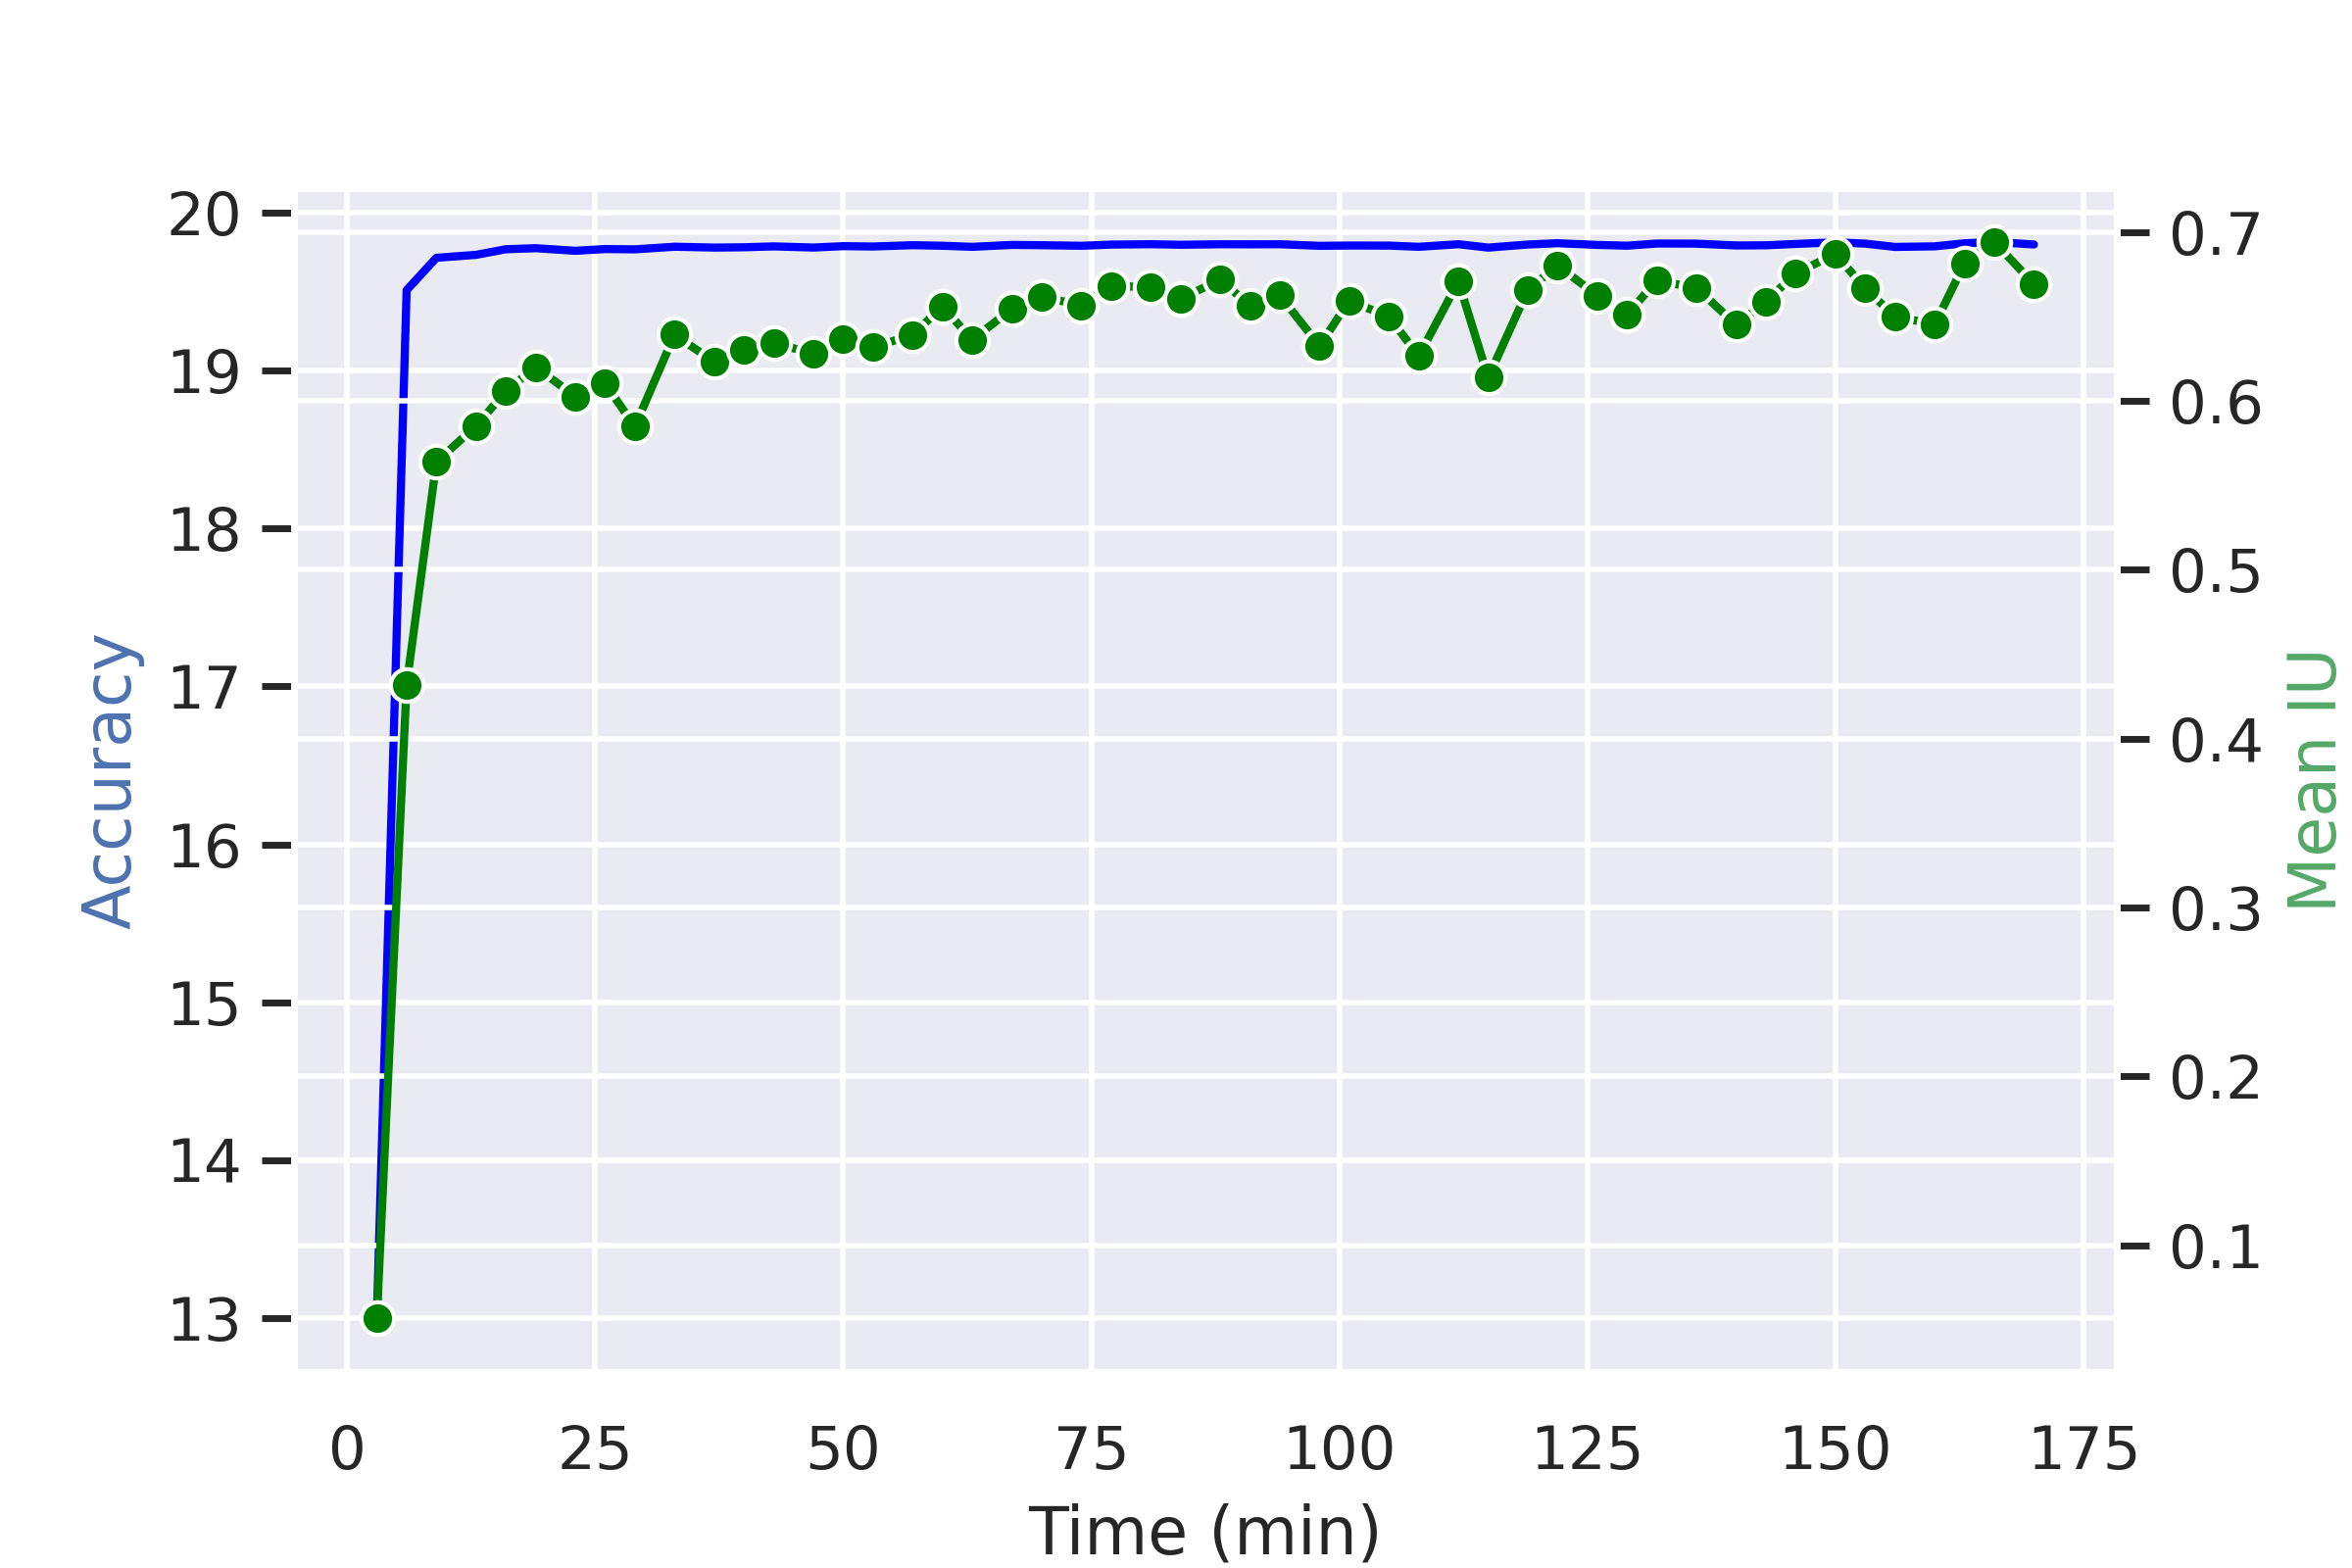
\includegraphics[width=0.6\textwidth]{annexes/graph/epoch_segtrain.png}
	    \caption{Le processus d'entraînement du modèle ArSeg}
	    \label{fig:epoch_mode}
	\end{figure}
	
	\begin{table}[]
	    \centering
        \begin{tabular}{|l|l|l|l|l|}
        \hline
        \multicolumn{1}{|c|}{\textbf{Model}} & \textbf{val\_acc} & \textbf{mean\_acc} & \textbf{mean\_iu} & \textbf{freq\_iu} \\ \hline
        \textbf{ArSeg}                       & 19.81395          & 19.81395           & 0.69404           & 0.69404           \\ \hline
        \end{tabular}
        \caption{Evaluation des performances du modèle ArSeg}
        \label{tab:ArSeg_benchmark}
    \end{table}
	
	L'entraînement sur nos documents historiques a été exécuter sur la base des recommandations établis par Juliette Janès et al. pour l'entraînement d'un modèle de mise en page\footcite{janesAutomaticTEIEncoding2021a}. La commande shell (retrouvable au sein de l'annexe D, voir \ref{code:segment}) reprend ainsi le réseau neuronal défini préalablement.
	
	Néanmoins, les résultats affichés durant l'entraînement démontrent de nombreuses fragilités. L'évaluation d'un modèle de segmentation s'est axé sur deux systèmes mesures : le \textit{mean Intersection-Over-Union} (Mean IU) qui reprend l'ensemble de l'indice de Jacard calculant la similarité entre deux éléments et le taux d'alignement;  le mean Accuracy calcule la moyenne de toutes les classes sur le principe de la métrique \gls{ACC}\footnote{Pour plus de détails, les explications faites par Hugo Scheithauer sont très explicites. \cite[p.~79-80]{scheithauerReconnaissanceEntitesNommees2021}}. 
	
	Comme le démontre la figure \ref{fig:segment_model}, les prédictions affichent un manque de régularité sur l'appréciation des \textit{baselines} et des zones. Les lignes en marge du document sont quant à elles ignorées ou très mal déterminées. De même, on observe que seules les zones \textit{Main:text} et \textit{QuireMarksZone:signature} sont identifiées. Ce dernier point peut démontrer le besoin de simplifier l'ontologie.
	
	\begin{figure}[p]
	    \centering
	    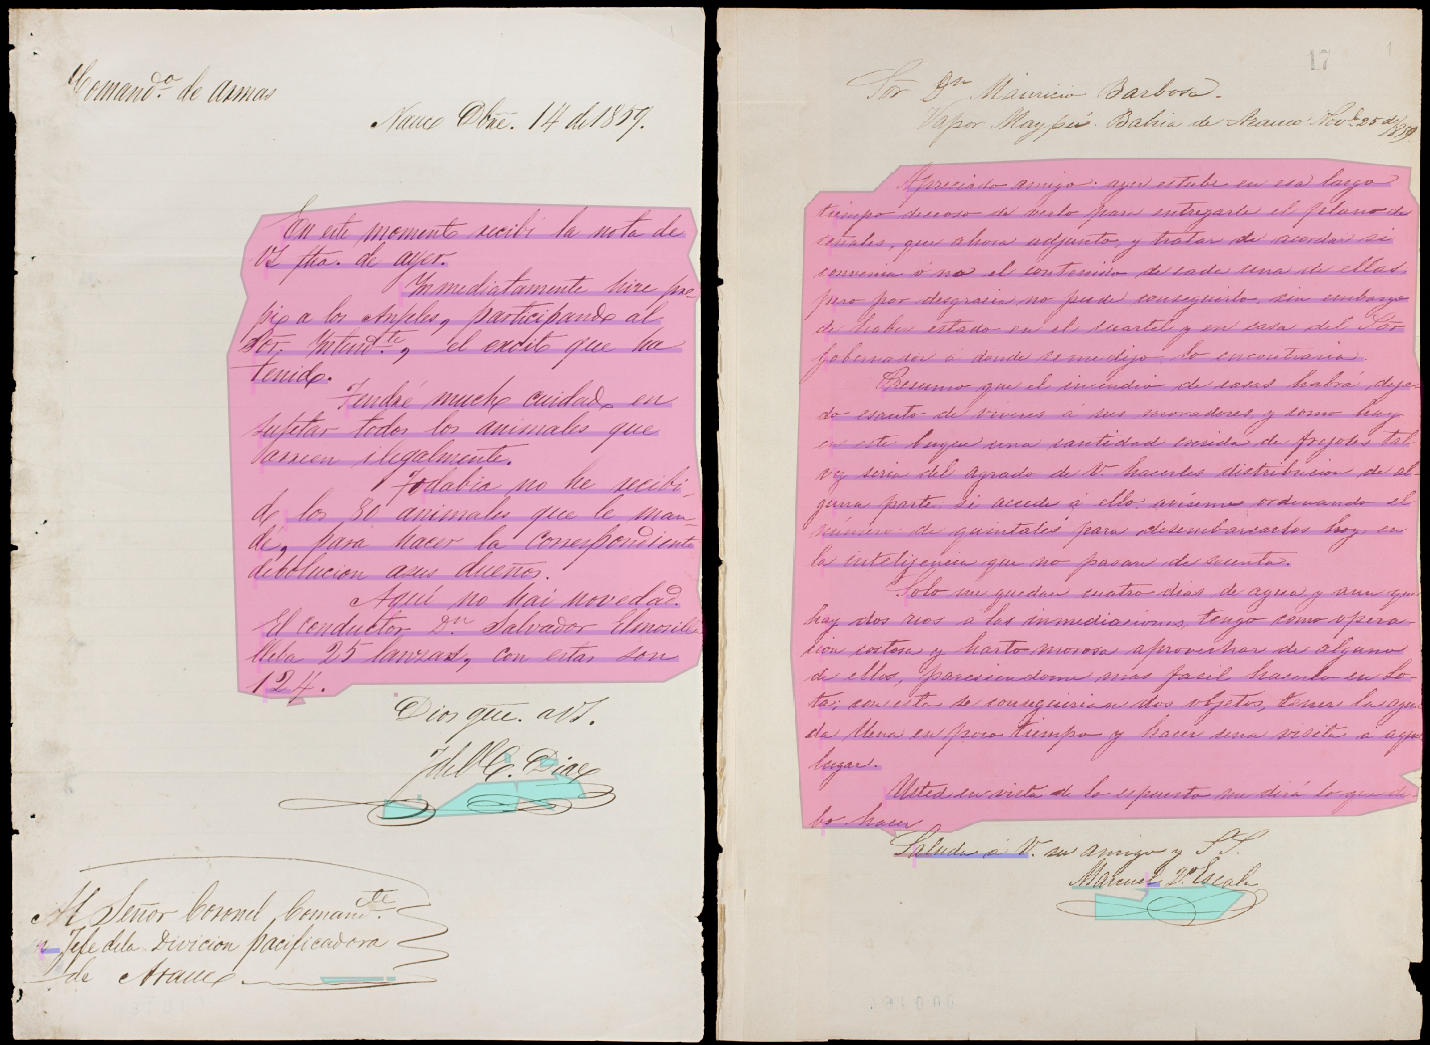
\includegraphics[width=1\textwidth]{annexes/img/segment_model.png}
	    \caption{Exemple de segmentation à partir du modèle ArSeg}
	    \label{fig:segment_model}
	\end{figure}
	
    Face à ce constat, le modèle ne permet pas d'obtenir une segmentation efficiente  et exploitable afin de l'intégrer au sein du flux éditorial. Une segmentation manuelle à partir du modèle par défaut proposé sur la plateforme \gls{eScriptorium} reste privilégiée au cours de cette chaîne de traitement afin de réévaluer les données d'entraînements.
    
	Les récents résultats présentés par Thibault Clérice peuvent laisser un espoir d'amélioration du système de segmentation\footcite{clericeYouActuallyLook2022}. Il propose de déplacer, par souci d'efficacité, la reconnaissance non plus sur une polygonisation basée sur la classification des pixels, mais à une détection d'objet utilisant des rectangles isothétiques. Pour cela, il appuie l'incorporation du moteur \texttt{YOLOv5} au sein du moteur \gls{kraken}.
	
	\section{La gestion des erreurs : le post-traitement comme second souffle à l'HTR}
	\sectionmark{Le post-traitement HTR}
	
	La reconnaissance automatique de texte ne s'arrête pas aux seuls prédictions du modèle \gls{htr}. Depuis les années 1990, de nombreux projets se sont appuyés sur le post-traitement des prédictions afin d'améliorer la qualité, en s'appuyant notamment sur des modèles statistiques aux frontières de la linguistique, en particulier les systèmes d'occurrences séquentielles (n-grammes) \footcite{takahashiSpellingCorrectionMethod1990, tongStatisticalApproachAutomatic1996}.
	
	Nous allons observer comment le projet Araucania a tenté de prolonger cette chaîne de traitement \gls{htr} en procédant à une mise en place d'une post-correction automatique. Le but est de réduire significativement les erreurs issues des transcriptions grâce à l'aide d'un corpus témoin.
	
	\subsection{Principe de la Distance de Levenshtein}
	
	Les erreurs des prédictions \gls{ocr} et \gls{htr} se résument à des erreurs de substitutions, d'insertions ou de suppressions de caractères au sein d'un ou plusieurs mots. Ces altérations au sein d'un mot transcrit peuvent être décrit à travers la distance de Levenshtein. Cette mesure de la différence entre deux chaînes de caractères a été proposée sous la forme d'un algorithme linguistique par le mathématicien russe Vladimir Levenshtein en 1965. Le principe y est assez simple, plus la distance est élevé, plus le mot transcrit a donc subi d'altérations. 
	
	\begin{wrapfigure}[7]{r}{9cm}
        \centering
        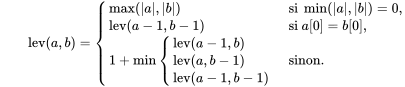
\includegraphics[width=7.5cm]{annexes/img/leventshein.png}
        \caption{Algorithme de Levenshtein - @wikipedia}
        \label{fig:algo_levenshtein}
    \end{wrapfigure}
    
    Dès la fin des années 1990, certains ingénieurs se sont essayer à intégrer cette distance dans leur chaîne de traitement \gls{ocr} afin d'estimer les candidats correctifs les plus prometteurs à partir de calculs probabilistes selon des séquences de caractères et de mots (n-grammes) texte\footcite{tongStatisticalApproachAutomatic1996}. Depuis, d'autres projets ont essayer d'intégrer cette mesure grâce à l'appui de dictionnaires d'occurrences, classification de mots, séquence de caractères notamment pour les problèmes de segmentations entre les mots\footcite{kissosOCRErrorCorrection2016, haldarLevenshteinDistanceTechnique}. Les différentes méthodes ont permis de réduire le nombre d'erreurs des prédictions \gls{ocr} jusqu'à 30\%. En ce sens, nous remarquons l'initiative du projet \gls{dahn} dirigé par Floriane Chiffoleau qui introduit une correction \textit{via} la distance de Levenshtein\footcite{chiffoleauDAHNProjectDigital2022}.
	
	\subsection{Mise en place d'une correction automatisée}
	
	Sur le modèle du projet \gls{dahn}, nous avons expérimenté la mise en place d'un CLI correctif au sein de la chaîne de traitement. Le script s'est fondé plus exactement sur l'incorporation de la librairie python \texttt{PySpellchecker}, et secondairement la librairie de \gls{tal} \gls{spacy} \footcite{barrusPyspellchecker2022}.
	
	\texttt{PySpellchecker} intègre un système de correction statistique à partir d'un dictionnaire d'occurrence, en appliquant la distance de Damerau-Levenshtein pour identifier les altérations possibles et une détermination des candidats grâce au théorème de Bayes, permettant de déterminer la probabilité d'un évènement par rapport à d'autres\footcite{norvigHowWriteSpelling2007}. L'idée est donc de générer l'ensemble des possibilités dans la limite de cette distance, et choisir le candidat le plus plausible. En ce sens, le dictionnaire d'occurrences permet de sélectionner le candidat à partir de ces calculs probabilistes, l'inférence bayésienne c'est-à-dire la démarche logique permettant de calculer ou actualiser la probabilité d'une hypothèse.\footcite[Récemment cette technique est encore recommandée, avec une amélioration de près de 30\% des cas comme le révèle cette étude.][]{haldarLevenshteinDistanceTechnique}.
	
	\begin{equation}
    \label{eq:bayes}
    P(\alpha|\beta) = \frac{P(\beta |\alpha)P(\alpha)}{P(\beta)}
    \end{equation}
    
    La complexité de la correction est décrite par un article publié en 2019 qui étudie statistiquement les erreurs récurrentes au sein des mécanismes \gls{ocr}\footcite{nguyenDeepStatisticalAnalysis2019}. Comme évoqué en amont, le groupe de chercheurs décrivent deux types d'erreurs fondamentales. La détection de ces erreurs multiples est corrélée à une distance plus grande, multipliant par conséquent le nombre de candidats possibles et donc accroissement du bruit. Au vu des résultats du modèle ArMcFR, nous avons estimé qu'une distance de 2 serait suffisante au vue d'une distance moyenne par mot assez faible (43) sur l'ensemble de la transcription, indiquant une répartition plus forte des erreurs (WER de 21\%). \newpar
    
    Comme l'indique le schéma du script suivant (voir figure \ref{fig:postprocess}), le processus s'est basé sur les recommandations de Daniel Lopresti dans la construction d'une chaîne de traitement post-OCR\footcite{loprestiOpticalCharacterRecognition2009}. Ligne par ligne, les phrases subissent un processus de tokénisation afin d'en révéler les informations essentielles, et de pouvoir traiter les mots individuellement. Le dictionnaire d'occurrences comme corpus de contrôle a ainsi été construit autour des données terrains produites précédemment afin d'aligner le niveau de langue de nos documents historiques avec nos prédictions \gls{htr}\footcite{humeauPostprocessHTR2022}. Les dictionnaires par défaut sont davantage adaptés aux corrections des productions très contemporaines.
	
	\begin{figure}[h!]
	    \centering
	    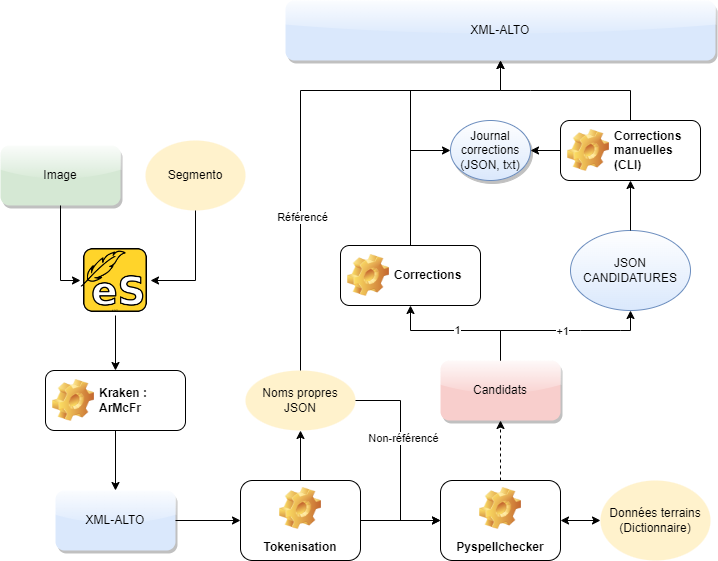
\includegraphics[width=0.8\textwidth]{annexes/schema/post_traitement.png}
	    \caption{Schéma de traitement des prédictions HTR}
	    \label{fig:postprocess}
	\end{figure}
	
	Une des premières étapes est de sélectionner les tokens dont la nature (POS, \textit{part of speech} en anglais) est un nom propre afin d'être identifiée au sein d'un répertoire de noms propres géographiques\footnote{Le dictionnaire JSON s'appuie sur un dictionnaire du XIX\textsuperscript{e} siècle : \cite{solanoasta-buruagaDiccionarioGeograficoRepublica1899}. Le dictionnaire a été produit \textit{via webscrapping} dont le script est disponible ici : \cite{humeauEnrichmentWikisource2022}}. S'il n'est pas détecté il est donc retourné comme erreur au sein du processus de correction. Ce procédé permet de pallier au limite du dictionnaire d'occurrences construit sur des données préalablement identifiées. Certains lieux lui sont donc encore inconnus, relevant ainsi d'une erreur.
    
    Selon les erreurs détectées et retournées, les candidats sont alors soumis à un processus de sélection restrictif, et ce en fonction d'une distance limite de 2 entre le mot identifié et les propositions faites. Si les propositions sont au nombre de 1 alors, le fichier \gls{alto} est automatiquement édité avec la correction sélectionnée. En revanche, si la liste des propositions est égale à zéro ou supérieure à 1 alors les données sont enregistrées au sein d'un fichier \gls{json} afin d'être corrigées manuellement.
	
	\subsection{Résultats et améliorations}
	
	Afin d'évaluer la performance du traitement correctif des fichiers \gls{htr}, nous avons réalisé une analyse textuelle comparative grâce à la librairie \texttt{KaMi-Lib} à partir d'un échantillon de quatre fichiers de notre jeu de données test. Les prédictions basiques ont été effectuées avec le modèle ArMcFr, puis comparées aux mêmes données transformées par le script de corrections. Malgré quelques tentatives d'améliorations, les résultats se sont montrés assez décevants pour le moment comme le montre le tableau de comparaison \ref{tab:erreurs_compa}. 
	
	Étonnamment, les premières mesures indiquent une augmentation des métriques \gls{CER} et \gls{WER} pouvant signaler une forte distorsion provoquée par la correction automatique. En revanche, les évaluations complémentaires indiquent une très légère progression concernant la distance entre la prédiction \gls{htr} et la correction proposée et les altérations de caractères. L'augmentation des mesures \gls{CER} et \gls{WER} pourraient donc s'expliquer par une réduction des caractères totaux et une plus forte disparité entre les mots corrigés positifs et les mots corrigés négatifs notamment à cause d'une mauvaise gestion des accents.
	
	\begin{table}[h]
	\centering
    \begin{tabular}{l|cc|c|}
    \cline{2-4}
                                        & \multicolumn{1}{l|}{\textbf{Prediction}} & \multicolumn{1}{l|}{\textbf{Correction}} & \multicolumn{1}{l|}{\textbf{Différence}} \\ \hline
    \multicolumn{1}{|l|}{CER (\%)}           & 13.58                                    & 13.77                                    & +0.19                                    \\ \cline{1-1} \hline
    \multicolumn{1}{|l|}{WER (\%)}           & 45.48                                    & 42.56                                    & +2.92                                    \\ \cline{1-1} \hline
    \multicolumn{1}{|l|}{D\textsubscript{mots}}   & 77                                       & 72                                       & -5                                       \\ \cline{1-1} \hline
    \multicolumn{1}{|l|}{Insertions}    & 13.25                                    & 11.25                                    & -2                                       \\ \cline{1-1} \hline
    \multicolumn{1}{|l|}{Deletions}     & 19.25                                    & 17                                       & -2.25                                    \\ \cline{1-1} \hline
    \multicolumn{1}{|l|}{Substitutions} & 91                                       & 87.75                                    & -3.25                                    \\ \cline{1-1} \hline
    \end{tabular}
    \caption{Analyse des effets du traitement automatique des erreurs HTR}
    \label{tab:erreurs_compa}
    \end{table}
    
    Nous pouvons émettre plusieurs constats d'améliorations à la suite de notre analyse de cas. La première difficulté réside dans la gestion des noms propres, et ce malgré le filtrage à partir du POS, dont la détermination se révèle souvent erronée. Dans de nombreux cas, les noms géographiques ont été abrégés au sein des transcriptions, complexifiant grandement l'opération de correction. L'autre point est la gestion dans sa globalité des noms propres comme le renseigne Hugo Scheithauer, après quelques expérimentations pour le projet \gls{lectaurep}\footcite[p.~88-89]{scheithauerReconnaissanceEntitesNommees2021}.
	
	La seconde difficulté, et sans doute la plus grande, réside dans la détection des erreurs au sein des mots réels (40\%)\footcite{nguyenDeepStatisticalAnalysis2019}. À l’inverse d'un mot non-réel, le mot réel signifie que les altérations DIS ont transformés le mot initial en un autre mot existant et référencé. Nous l'avons vu, l'orthographe est très variable et ponctuée de fautes au sein des archives. Ces différences linguistiques amènent donc une difficulté à identifier les erreurs \gls{htr} avec les variations orthographiques et les erreurs orthographiques originales. De plus, ces variations, volontaires ou non, augmentent artificiellement le nombre de mots existants, biaisant le dictionnaire d'occurrences et donc les probabilités bayésiennes. Une solution pourrait s'imaginer avec l'introduction d'un processus de lemmatisation entre le produit \gls{htr} et le corpus contrôle, et une meilleure utilisation de l'étiquetage de la parole (POS). \newpar
	
	Comme signalé par Youness Chaabi et Fadoua Ataa Allah, le système Norving employé par la librairie \texttt{PySpellchecker} possède de nombreuses limites\footcite{chaabiAmazighSpellChecker2022}. Le système de classification par dictionnaire d'occurrences est éprouvé depuis très longtemps qui bien que conçu pour être effectué au travers de calcul simple, celui-ci est connu pour générer un trop gros nombre de résultats\footnote{Même si le nombre est alors limité par la définition de la distance de Levenshtein.}. De plus, l'effet de contextualisation du mot erroné au sein de la phrase est assez limité. En ce sens, une combinaison entre le système Norvik et l'utilisation de l'analyse séquentielle par N-grammes pourrait permettre l'obtention de meilleurs résultats comme le proposent les chercheurs de l'Université du Roi-Saoud\footcite{chaabiAmazighSpellChecker2022}.
	
    Lors du concours de l'IDCAR 2019, l'utilisation de cette architecture est remarquée puisque le modèle BERT démontre un fort potentiel dans la résolution de correction contextuelle\footcite{rigaudICDAR2019Competition2019}. Par la suite, plusieurs groupes de chercheurs ont mis à profit ces résultats primaires afin de construire de nouvelles expérimentations avec les architectures \gls{tal} encodeurs-décodeurs (BERT, RoBERTa, etc.)\footcite{palVartaniSpellcheckAutomatic2020, karthikeyanOCRPostCorrectionApproach2022}. Les projets mettent à contribution la recherche d'entités-nommées et les vecteurs de mots afin de prédire le mot correct caché par le système du masque. Les résultats obtenus notamment par l'Université de l'Essex indiquent une réduction substantielle des erreurs faites par la prédiction \gls{ocr}\footcite{karthikeyanOCRPostCorrectionApproach2022}. Toutefois, la mise en place de ce système exige des ressources matérielles bien plus importantes. 